\PassOptionsToPackage{unicode=true}{hyperref} % options for packages loaded elsewhere
\PassOptionsToPackage{hyphens}{url}
%
\documentclass[]{article}
\usepackage{lmodern}
\usepackage{amssymb,amsmath}
\usepackage{ifxetex,ifluatex}
\usepackage{fixltx2e} % provides \textsubscript
\ifnum 0\ifxetex 1\fi\ifluatex 1\fi=0 % if pdftex
  \usepackage[T1]{fontenc}
  \usepackage[utf8]{inputenc}
  \usepackage{textcomp} % provides euro and other symbols
\else % if luatex or xelatex
  \usepackage{unicode-math}
  \defaultfontfeatures{Ligatures=TeX,Scale=MatchLowercase}
\fi
% use upquote if available, for straight quotes in verbatim environments
\IfFileExists{upquote.sty}{\usepackage{upquote}}{}
% use microtype if available
\IfFileExists{microtype.sty}{%
\usepackage[]{microtype}
\UseMicrotypeSet[protrusion]{basicmath} % disable protrusion for tt fonts
}{}
\IfFileExists{parskip.sty}{%
\usepackage{parskip}
}{% else
\setlength{\parindent}{0pt}
\setlength{\parskip}{6pt plus 2pt minus 1pt}
}
\usepackage{hyperref}
\hypersetup{
            pdfauthor={Joaquín Moreno1,2; Sergio Asensio2; Miguel Berdugo2,3; Beatriz Gozalo2; Victoria Ochoa2; Blas M. Benito2; Fernando T. Maestre2,4},
            pdfborder={0 0 0},
            breaklinks=true}
\urlstyle{same}  % don't use monospace font for urls
\usepackage[margin=1in]{geometry}
\usepackage{color}
\usepackage{fancyvrb}
\newcommand{\VerbBar}{|}
\newcommand{\VERB}{\Verb[commandchars=\\\{\}]}
\DefineVerbatimEnvironment{Highlighting}{Verbatim}{commandchars=\\\{\}}
% Add ',fontsize=\small' for more characters per line
\usepackage{framed}
\definecolor{shadecolor}{RGB}{248,248,248}
\newenvironment{Shaded}{\begin{snugshade}}{\end{snugshade}}
\newcommand{\AlertTok}[1]{\textcolor[rgb]{0.94,0.16,0.16}{#1}}
\newcommand{\AnnotationTok}[1]{\textcolor[rgb]{0.56,0.35,0.01}{\textbf{\textit{#1}}}}
\newcommand{\AttributeTok}[1]{\textcolor[rgb]{0.77,0.63,0.00}{#1}}
\newcommand{\BaseNTok}[1]{\textcolor[rgb]{0.00,0.00,0.81}{#1}}
\newcommand{\BuiltInTok}[1]{#1}
\newcommand{\CharTok}[1]{\textcolor[rgb]{0.31,0.60,0.02}{#1}}
\newcommand{\CommentTok}[1]{\textcolor[rgb]{0.56,0.35,0.01}{\textit{#1}}}
\newcommand{\CommentVarTok}[1]{\textcolor[rgb]{0.56,0.35,0.01}{\textbf{\textit{#1}}}}
\newcommand{\ConstantTok}[1]{\textcolor[rgb]{0.00,0.00,0.00}{#1}}
\newcommand{\ControlFlowTok}[1]{\textcolor[rgb]{0.13,0.29,0.53}{\textbf{#1}}}
\newcommand{\DataTypeTok}[1]{\textcolor[rgb]{0.13,0.29,0.53}{#1}}
\newcommand{\DecValTok}[1]{\textcolor[rgb]{0.00,0.00,0.81}{#1}}
\newcommand{\DocumentationTok}[1]{\textcolor[rgb]{0.56,0.35,0.01}{\textbf{\textit{#1}}}}
\newcommand{\ErrorTok}[1]{\textcolor[rgb]{0.64,0.00,0.00}{\textbf{#1}}}
\newcommand{\ExtensionTok}[1]{#1}
\newcommand{\FloatTok}[1]{\textcolor[rgb]{0.00,0.00,0.81}{#1}}
\newcommand{\FunctionTok}[1]{\textcolor[rgb]{0.00,0.00,0.00}{#1}}
\newcommand{\ImportTok}[1]{#1}
\newcommand{\InformationTok}[1]{\textcolor[rgb]{0.56,0.35,0.01}{\textbf{\textit{#1}}}}
\newcommand{\KeywordTok}[1]{\textcolor[rgb]{0.13,0.29,0.53}{\textbf{#1}}}
\newcommand{\NormalTok}[1]{#1}
\newcommand{\OperatorTok}[1]{\textcolor[rgb]{0.81,0.36,0.00}{\textbf{#1}}}
\newcommand{\OtherTok}[1]{\textcolor[rgb]{0.56,0.35,0.01}{#1}}
\newcommand{\PreprocessorTok}[1]{\textcolor[rgb]{0.56,0.35,0.01}{\textit{#1}}}
\newcommand{\RegionMarkerTok}[1]{#1}
\newcommand{\SpecialCharTok}[1]{\textcolor[rgb]{0.00,0.00,0.00}{#1}}
\newcommand{\SpecialStringTok}[1]{\textcolor[rgb]{0.31,0.60,0.02}{#1}}
\newcommand{\StringTok}[1]{\textcolor[rgb]{0.31,0.60,0.02}{#1}}
\newcommand{\VariableTok}[1]{\textcolor[rgb]{0.00,0.00,0.00}{#1}}
\newcommand{\VerbatimStringTok}[1]{\textcolor[rgb]{0.31,0.60,0.02}{#1}}
\newcommand{\WarningTok}[1]{\textcolor[rgb]{0.56,0.35,0.01}{\textbf{\textit{#1}}}}
\usepackage{graphicx,grffile}
\makeatletter
\def\maxwidth{\ifdim\Gin@nat@width>\linewidth\linewidth\else\Gin@nat@width\fi}
\def\maxheight{\ifdim\Gin@nat@height>\textheight\textheight\else\Gin@nat@height\fi}
\makeatother
% Scale images if necessary, so that they will not overflow the page
% margins by default, and it is still possible to overwrite the defaults
% using explicit options in \includegraphics[width, height, ...]{}
\setkeys{Gin}{width=\maxwidth,height=\maxheight,keepaspectratio}
\setlength{\emergencystretch}{3em}  % prevent overfull lines
\providecommand{\tightlist}{%
  \setlength{\itemsep}{0pt}\setlength{\parskip}{0pt}}
\setcounter{secnumdepth}{5}
% Redefines (sub)paragraphs to behave more like sections
\ifx\paragraph\undefined\else
\let\oldparagraph\paragraph
\renewcommand{\paragraph}[1]{\oldparagraph{#1}\mbox{}}
\fi
\ifx\subparagraph\undefined\else
\let\oldsubparagraph\subparagraph
\renewcommand{\subparagraph}[1]{\oldsubparagraph{#1}\mbox{}}
\fi

% set default figure placement to htbp
\makeatletter
\def\fps@figure{htbp}
\makeatother

\usepackage{booktabs}
\usepackage[table]{xcolor}
\usepackage{color}
\usepackage{fontspec}
\setmainfont[Scale=1.1]{Open Sans}
\setmonofont[Scale=0.9]{Open Sans}
\linespread{1.3}
\usepackage{listings}
\lstset{breaklines=true}

\usepackage{float}
\let\origfigure\figure
\let\endorigfigure\endfigure
\renewenvironment{figure}[1][2] {
    \expandafter\origfigure\expandafter[H]
} {
    \endorigfigure
}

\floatplacement{figure}{H}

\usepackage{pdflscape}
\newcommand{\blandscape}{\begin{landscape}}
\newcommand{\elandscape}{\end{landscape}}

\usepackage{caption} 
\captionsetup[table]{skip=10pt}
\usepackage[tableposition=above]{caption}

\title{The MOISCRUST dataset:\\
a spatio-temporal continuous soil moisture dataset\\
from a Mediterranean semiarid dryland\\
from 2006 to 2020\\
~\\
SUPPLEMENTARY MATERIAL}
\author{Joaquín Moreno\textsuperscript{1,2} \and Sergio Asensio\textsuperscript{2} \and Miguel Berdugo\textsuperscript{2,3} \and Beatriz Gozalo\textsuperscript{2} \and Victoria Ochoa\textsuperscript{2} \and Blas M. Benito\textsuperscript{2} \and Fernando T. Maestre\textsuperscript{2,4}}
\date{}

\begin{document}
\maketitle

{
\setcounter{tocdepth}{2}
\tableofcontents
}
\textsuperscript{1} Corresponding author, e-mail:
\href{mailto:joaquin.moreno@ua.es}{\nolinkurl{joaquin.moreno@ua.es}}\\
\textsuperscript{2} Instituto Multidisciplinar para el Estudio del Medio
``Ramon Margalef'', Universidad de Alicante, Edificio Nuevos Institutos,
Carretera de San Vicente del Raspeig s/n, 03690 San Vicente del Raspeig,
Spain.\\
\textsuperscript{3} Institut Department of Environmental Systems
Science, ETH Zürich. Universitätstrasse 16, 8092 Zurich, Switzerland.\\
\textsuperscript{4} Departamento de Ecología, Universidad de Alicante,
Carretera de San Vicente del Raspeig s/n, 03690 San Vicente del Raspeig,
Alicante, Spain.

\hypertarget{summary}{%
\section{Summary}\label{summary}}

XXX

\hypertarget{installing-and-loading-the-required-libraries}{%
\section{Installing and loading the required
libraries}\label{installing-and-loading-the-required-libraries}}

The following libraries are required to run this workflow. These are
already installed in the local \texttt{renv} folder, so there is no need
to install them if you don't have them in your computer.

\begin{Shaded}
\begin{Highlighting}[]
\CommentTok{#automatic install of packages if they are not readily available}
\NormalTok{required_packages <-}\StringTok{ }\KeywordTok{c}\NormalTok{(}
  \StringTok{"data.table"}\NormalTok{,}
  \StringTok{"janitor"}\NormalTok{,}
  \StringTok{"tidyverse"}\NormalTok{,}
  \StringTok{"kableExtra"}\NormalTok{,}
  \StringTok{"foreach"}\NormalTok{,}
  \StringTok{"doParallel"}\NormalTok{,}
  \StringTok{"readr"}\NormalTok{,}
  \StringTok{"writexl"}\NormalTok{,}
  \StringTok{"RSQLite"}\NormalTok{,}
  \StringTok{"zip"}\NormalTok{,}
  \StringTok{"knitr"}
\NormalTok{)}

\CommentTok{#loading packages}
\KeywordTok{invisible}\NormalTok{(}\KeywordTok{lapply}\NormalTok{(required_packages, library, }\DataTypeTok{character.only =} \OtherTok{TRUE}\NormalTok{))}

\CommentTok{#removing objects}
\KeywordTok{rm}\NormalTok{(required_packages)}

\CommentTok{#knitr options}
\NormalTok{knitr}\OperatorTok{::}\NormalTok{opts_chunk}\OperatorTok{$}\KeywordTok{set}\NormalTok{(}\DataTypeTok{echo =} \OtherTok{TRUE}\NormalTok{, }\DataTypeTok{warning =} \OtherTok{FALSE}\NormalTok{, }\DataTypeTok{message =} \OtherTok{FALSE}\NormalTok{)}
\NormalTok{knitr}\OperatorTok{::}\NormalTok{knit_hooks}\OperatorTok{$}\KeywordTok{set}\NormalTok{(}\DataTypeTok{document =} \ControlFlowTok{function}\NormalTok{(x) \{}\KeywordTok{sub}\NormalTok{(}\StringTok{'}\CharTok{\textbackslash{}\textbackslash{}}\StringTok{usepackage\{xcolor\}'}\NormalTok{, }\StringTok{'}\CharTok{\textbackslash{}\textbackslash{}}\StringTok{usepackage\{xcolor\}'}\NormalTok{, x, }\DataTypeTok{fixed =} \OtherTok{TRUE}\NormalTok{)\})}
\end{Highlighting}
\end{Shaded}

\hypertarget{data-loading-and-preparation}{%
\section{Data loading and
preparation}\label{data-loading-and-preparation}}

\hypertarget{loading-the-data}{%
\subsection{Loading the data}\label{loading-the-data}}

\begin{Shaded}
\begin{Highlighting}[]
\CommentTok{#load, clean names, and rename time columns}
\NormalTok{moiscrust <-}\StringTok{ }\NormalTok{data.table}\OperatorTok{::}\KeywordTok{fread}\NormalTok{(}\DataTypeTok{file =} \StringTok{"moiscrust_raw.csv"}\NormalTok{) }\OperatorTok\StringTok{ }
\StringTok{  }\NormalTok{janitor}\OperatorTok{::}\KeywordTok{clean_names}\NormalTok{() }\OperatorTok\StringTok{ }
\StringTok{  }\NormalTok{dplyr}\OperatorTok{::}\KeywordTok{rename}\NormalTok{(}
    \DataTypeTok{date =}\NormalTok{ dates,}
    \DataTypeTok{time =}\NormalTok{ hour}
\NormalTok{    ) }\OperatorTok\StringTok{ }
\StringTok{  }\KeywordTok{as.data.frame}\NormalTok{()}
\end{Highlighting}
\end{Shaded}

\hypertarget{formatting-dates-and-times}{%
\subsection{Formatting dates and
times}\label{formatting-dates-and-times}}

\begin{Shaded}
\begin{Highlighting}[]
\CommentTok{#date to Year-month-day}
\NormalTok{moiscrust}\OperatorTok{$}\NormalTok{date <-}\StringTok{ }\KeywordTok{format}\NormalTok{(}
  \KeywordTok{as.POSIXct}\NormalTok{(}
    \KeywordTok{strptime}\NormalTok{(}
\NormalTok{      moiscrust}\OperatorTok{$}\NormalTok{date,}
      \StringTok{"%d/%m/%Y"}\NormalTok{,}
      \DataTypeTok{tz =} \StringTok{""}
\NormalTok{      )}
\NormalTok{    ),}
  \DataTypeTok{format =} \StringTok{"%Y-%m-%d"}
\NormalTok{  )}

\CommentTok{#time to Hour-Minute}
\NormalTok{moiscrust}\OperatorTok{$}\NormalTok{time <-}\StringTok{ }\KeywordTok{format}\NormalTok{(}
  \KeywordTok{as.POSIXct}\NormalTok{(}
    \KeywordTok{strptime}\NormalTok{(}
\NormalTok{      moiscrust}\OperatorTok{$}\NormalTok{time,}
      \StringTok{"%H:%M:%S"}\NormalTok{,}
      \DataTypeTok{tz =} \StringTok{""}
\NormalTok{      )}
\NormalTok{    ),}
  \DataTypeTok{format =} \StringTok{"%H:%M"}
\NormalTok{  )}

\CommentTok{#joining date and time}
\NormalTok{moiscrust}\OperatorTok{$}\NormalTok{date_time <-}\StringTok{ }\KeywordTok{as.POSIXct}\NormalTok{(}
  \KeywordTok{paste}\NormalTok{(}
\NormalTok{    moiscrust}\OperatorTok{$}\NormalTok{date, }
\NormalTok{    moiscrust}\OperatorTok{$}\NormalTok{time}
\NormalTok{    ), }
  \DataTypeTok{format=}\StringTok{"%Y-%m-%d %H:%M"}
\NormalTok{  )}

\CommentTok{#unique id for each observation}
\NormalTok{moiscrust}\OperatorTok{$}\NormalTok{date_time_id <-}\StringTok{ }\DecValTok{1}\OperatorTok{:}\KeywordTok{nrow}\NormalTok{(moiscrust)}

\CommentTok{#creating year, month, and day related columns}
\NormalTok{moiscrust}\OperatorTok{$}\NormalTok{year <-}\StringTok{ }\NormalTok{lubridate}\OperatorTok{::}\KeywordTok{year}\NormalTok{(moiscrust}\OperatorTok{$}\NormalTok{date)}
\NormalTok{moiscrust}\OperatorTok{$}\NormalTok{year_day <-}\StringTok{ }\NormalTok{lubridate}\OperatorTok{::}\KeywordTok{yday}\NormalTok{(moiscrust}\OperatorTok{$}\NormalTok{date)}
\NormalTok{moiscrust}\OperatorTok{$}\NormalTok{month <-}\StringTok{ }\NormalTok{lubridate}\OperatorTok{::}\KeywordTok{month}\NormalTok{(moiscrust}\OperatorTok{$}\NormalTok{date)}
\NormalTok{moiscrust}\OperatorTok{$}\NormalTok{month_day <-}\StringTok{ }\NormalTok{lubridate}\OperatorTok{::}\KeywordTok{mday}\NormalTok{(moiscrust}\OperatorTok{$}\NormalTok{date)}
\NormalTok{moiscrust}\OperatorTok{$}\NormalTok{week <-}\StringTok{ }\NormalTok{lubridate}\OperatorTok{::}\KeywordTok{week}\NormalTok{(moiscrust}\OperatorTok{$}\NormalTok{date)}
\NormalTok{moiscrust}\OperatorTok{$}\NormalTok{week_day <-}\StringTok{ }\NormalTok{lubridate}\OperatorTok{::}\KeywordTok{wday}\NormalTok{(moiscrust}\OperatorTok{$}\NormalTok{date)}
\end{Highlighting}
\end{Shaded}

\hypertarget{reordering-columns}{%
\subsection{Reordering columns}\label{reordering-columns}}

\begin{Shaded}
\begin{Highlighting}[]
\CommentTok{#names of the sensors}
\NormalTok{sensors <-}\StringTok{ }\KeywordTok{c}\NormalTok{(}
  \StringTok{"retama5094"}\NormalTok{,}
  \StringTok{"retama5062"}\NormalTok{,}
  \StringTok{"retama5063"}\NormalTok{,}
  \StringTok{"stipa5094"}\NormalTok{,}
  \StringTok{"stipa5062"}\NormalTok{,}
  \StringTok{"stipa5063"}\NormalTok{,}
  \StringTok{"bs_cl5094"}\NormalTok{,}
  \StringTok{"bs_cl5062"}\NormalTok{,}
  \StringTok{"bs_cl5063"}\NormalTok{,}
  \StringTok{"bs_cm5094"}\NormalTok{,}
  \StringTok{"bs_cm5062"}\NormalTok{,}
  \StringTok{"bs_cm5063"}\NormalTok{,}
  \StringTok{"bs_ch5094"}\NormalTok{,}
  \StringTok{"bs_ch5062"}\NormalTok{,}
  \StringTok{"bs_ch5063"}
\NormalTok{)}

\CommentTok{#reordering columns of moiscrust to have time in the left side}
\NormalTok{moiscrust <-}\StringTok{ }\NormalTok{moiscrust[, }\KeywordTok{c}\NormalTok{(}
  \StringTok{"date_time"}\NormalTok{,}
  \StringTok{"date_time_id"}\NormalTok{,}
  \StringTok{"date"}\NormalTok{,}
  \StringTok{"time"}\NormalTok{,}
  \StringTok{"year"}\NormalTok{,}
  \StringTok{"year_day"}\NormalTok{,}
  \StringTok{"month"}\NormalTok{,}
  \StringTok{"month_day"}\NormalTok{,}
  \StringTok{"week"}\NormalTok{,}
  \StringTok{"week_day"}\NormalTok{,}
\NormalTok{  sensors}
\NormalTok{)]}
\end{Highlighting}
\end{Shaded}

\hypertarget{to-long-format}{%
\subsection{To long format}\label{to-long-format}}

\begin{Shaded}
\begin{Highlighting}[]
\CommentTok{#to long format}
\NormalTok{moiscrust_long <-}\StringTok{ }\NormalTok{tidyr}\OperatorTok{::}\KeywordTok{pivot_longer}\NormalTok{(}
\NormalTok{  moiscrust,}
  \DataTypeTok{cols =} \KeywordTok{all_of}\NormalTok{(sensors),}
  \DataTypeTok{names_to =} \StringTok{"sensor"}\NormalTok{,}
  \DataTypeTok{values_to =} \StringTok{"soil_moisture"}
\NormalTok{)}
\end{Highlighting}
\end{Shaded}

\hypertarget{data-visualization}{%
\subsection{Data visualization}\label{data-visualization}}

\begin{Shaded}
\begin{Highlighting}[]
\KeywordTok{ggplot}\NormalTok{(moiscrust_long) }\OperatorTok{+}\StringTok{ }
\StringTok{  }\KeywordTok{facet_wrap}\NormalTok{(}\StringTok{"year"}\NormalTok{, }\DataTypeTok{scales =} \StringTok{"free_x"}\NormalTok{, }\DataTypeTok{ncol =} \DecValTok{2}\NormalTok{) }\OperatorTok{+}
\StringTok{  }\KeywordTok{aes}\NormalTok{(}\DataTypeTok{x =}\NormalTok{ year_day, }\DataTypeTok{y =}\NormalTok{ sensor, }\DataTypeTok{fill =}\NormalTok{ soil_moisture) }\OperatorTok{+}\StringTok{ }
\StringTok{  }\KeywordTok{geom_tile}\NormalTok{() }\OperatorTok{+}\StringTok{ }
\StringTok{  }\KeywordTok{coord_cartesian}\NormalTok{(}\DataTypeTok{expand =} \OtherTok{FALSE}\NormalTok{) }\OperatorTok{+}
\StringTok{  }\KeywordTok{theme_bw}\NormalTok{() }\OperatorTok{+}\StringTok{ }
\StringTok{  }\KeywordTok{scale_fill_viridis_c}\NormalTok{(}\DataTypeTok{direction =} \DecValTok{-1}\NormalTok{, }\DataTypeTok{na.value =} \StringTok{"white"}\NormalTok{, }\DataTypeTok{option =} \StringTok{"B"}\NormalTok{) }\OperatorTok{+}\StringTok{ }
\StringTok{  }\KeywordTok{theme}\NormalTok{(}\DataTypeTok{legend.position =} \StringTok{"bottom"}\NormalTok{) }\OperatorTok{+}\StringTok{ }
\StringTok{  }\KeywordTok{ylab}\NormalTok{(}\StringTok{""}\NormalTok{) }\OperatorTok{+}\StringTok{ }
\StringTok{  }\KeywordTok{xlab}\NormalTok{(}\StringTok{"Day of the year"}\NormalTok{) }\OperatorTok{+}
\StringTok{  }\KeywordTok{ggtitle}\NormalTok{(}\StringTok{"MOISCRUST database (raw data)"}\NormalTok{) }\OperatorTok{+}
\StringTok{  }\KeywordTok{labs}\NormalTok{(}\DataTypeTok{fill =} \KeywordTok{expression}\NormalTok{(}\StringTok{"Volumetric water content (cm³ water / cm³ soil)"}\NormalTok{)) }\OperatorTok{+}\StringTok{ }
\StringTok{  }\KeywordTok{theme}\NormalTok{(}\DataTypeTok{legend.key.width =} \KeywordTok{unit}\NormalTok{(}\DecValTok{1}\NormalTok{, }\StringTok{"cm"}\NormalTok{))}
\end{Highlighting}
\end{Shaded}

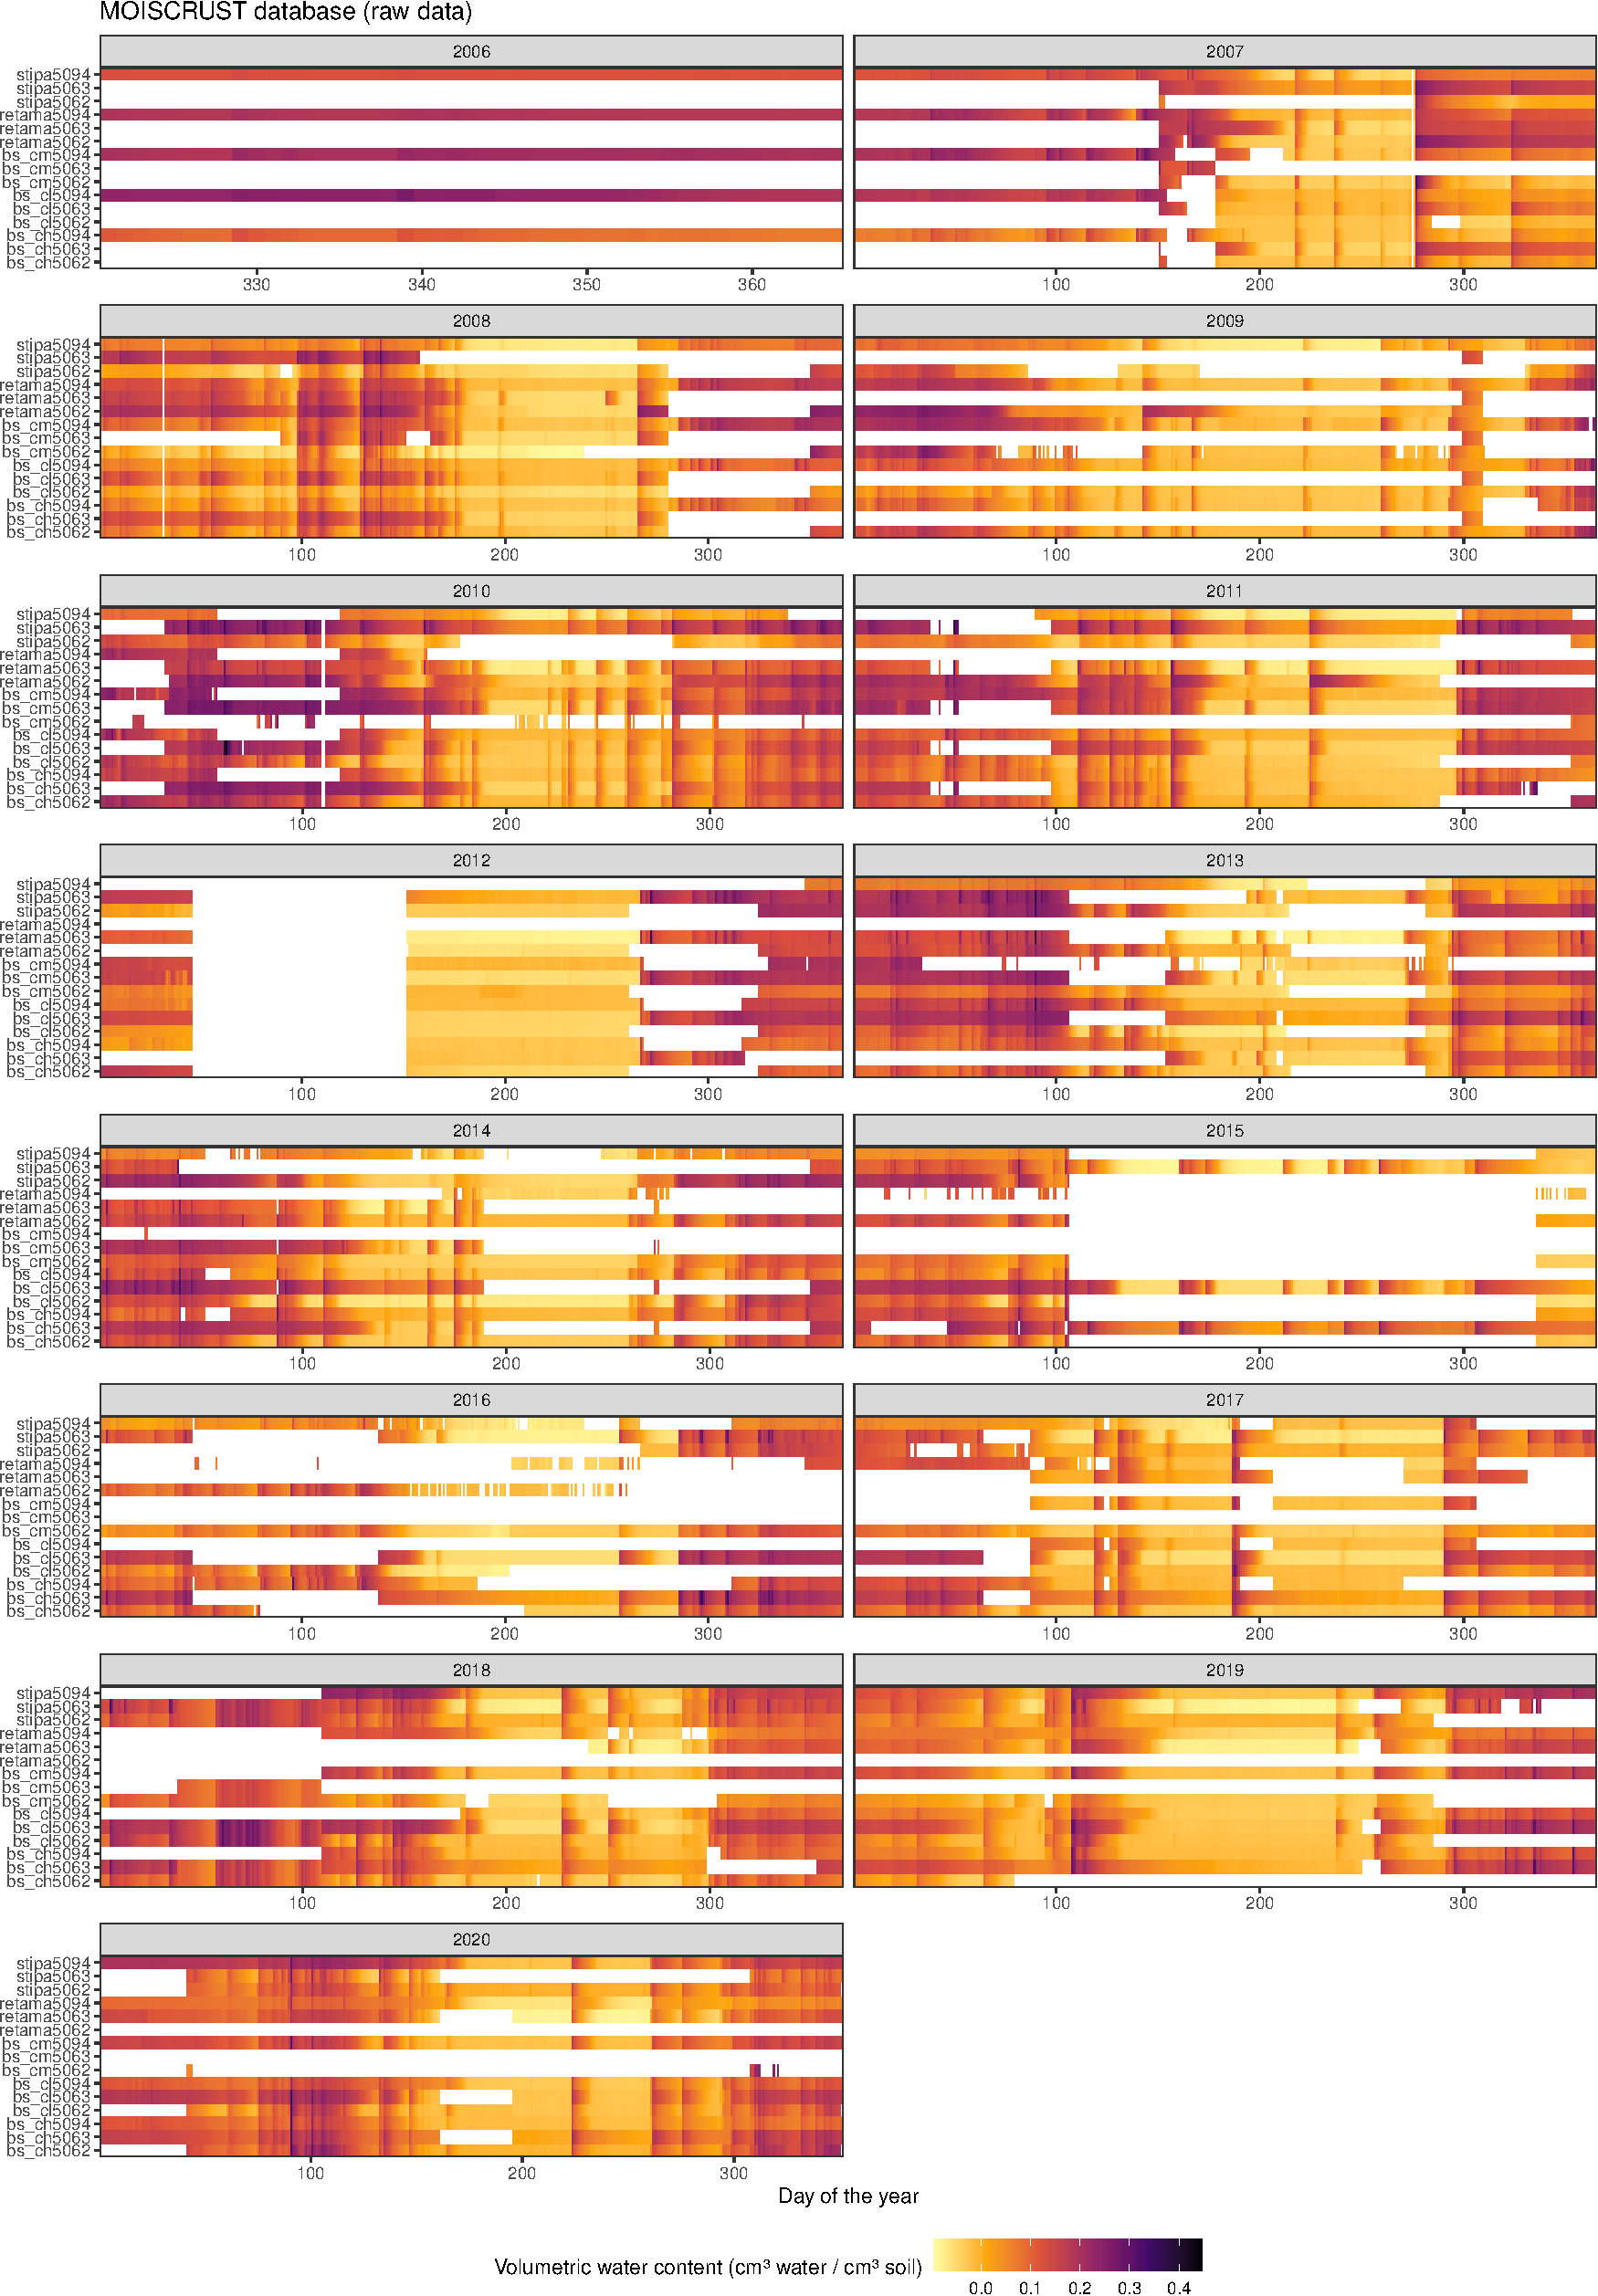
\includegraphics{moiscrust_files/figure-latex/unnamed-chunk-6-1.pdf}

\begin{Shaded}
\begin{Highlighting}[]
\KeywordTok{ggsave}\NormalTok{(}\DataTypeTok{width =} \DecValTok{12}\NormalTok{, }\DataTypeTok{height =} \DecValTok{17}\NormalTok{, }\DataTypeTok{filename =} \StringTok{"MOISCRUST_raw.pdf"}\NormalTok{)}
\end{Highlighting}
\end{Shaded}

\hypertarget{number-of-na-per-time-series}{%
\subsection{Number of NA per
time-series}\label{number-of-na-per-time-series}}

\begin{Shaded}
\begin{Highlighting}[]
\CommentTok{#counting NA values per sensor}
\NormalTok{moiscrust_NA <-}\StringTok{ }\NormalTok{moiscrust_long }\OperatorTok\StringTok{ }
\StringTok{  }\KeywordTok{group_by}\NormalTok{(sensor) }\OperatorTok\StringTok{ }
\StringTok{  }\KeywordTok{summarise}\NormalTok{(}\DataTypeTok{na_count =} \KeywordTok{sum}\NormalTok{(}\KeywordTok{is.na}\NormalTok{(soil_moisture))) }\OperatorTok\StringTok{ }
\StringTok{  }\KeywordTok{mutate}\NormalTok{(}\DataTypeTok{na_count_percent =} \KeywordTok{round}\NormalTok{((na_count }\OperatorTok{*}\StringTok{ }\DecValTok{100}\NormalTok{) }\OperatorTok{/}\StringTok{ }\KeywordTok{nrow}\NormalTok{(moiscrust), }\DecValTok{1}\NormalTok{))}

\CommentTok{#adding sensor sensor_group to the moiscrust_NA data frame}
\NormalTok{moiscrust_NA}\OperatorTok{$}\NormalTok{sensor_group <-}\StringTok{ }\KeywordTok{c}\NormalTok{(}
  \StringTok{"biocrust_high"}\NormalTok{,}
  \StringTok{"biocrust_high"}\NormalTok{,}
  \StringTok{"biocrust_high"}\NormalTok{,}
  \StringTok{"biocrust_low"}\NormalTok{,}
  \StringTok{"biocrust_low"}\NormalTok{,}
  \StringTok{"biocrust_low"}\NormalTok{,}
  \StringTok{"biocrust_medium"}\NormalTok{,}
  \StringTok{"biocrust_medium"}\NormalTok{,}
  \StringTok{"biocrust_medium"}\NormalTok{,}
  \StringTok{"retama"}\NormalTok{,}
  \StringTok{"retama"}\NormalTok{,}
  \StringTok{"retama"}\NormalTok{,}
  \StringTok{"stipa"}\NormalTok{,}
  \StringTok{"stipa"}\NormalTok{,}
  \StringTok{"stipa"}
\NormalTok{)}

\CommentTok{#reordering columns and arranging by na_count}
\NormalTok{moiscrust_NA <-}\StringTok{ }\NormalTok{moiscrust_NA[, }\KeywordTok{c}\NormalTok{(}
  \StringTok{"sensor"}\NormalTok{, }
  \StringTok{"sensor_group"}\NormalTok{, }
  \StringTok{"na_count"}\NormalTok{, }
  \StringTok{"na_count_percent"}
\NormalTok{  )] }\OperatorTok\StringTok{ }
\StringTok{  }\NormalTok{dplyr}\OperatorTok{::}\KeywordTok{arrange}\NormalTok{(na_count) }\OperatorTok\StringTok{ }
\StringTok{  }\KeywordTok{as.data.frame}\NormalTok{()}

\CommentTok{#showing the table}
\NormalTok{kableExtra}\OperatorTok{::}\KeywordTok{kbl}\NormalTok{(moiscrust_NA)}
\end{Highlighting}
\end{Shaded}

\begin{tabular}[t]{l|l|r|r}
\hline
sensor & sensor\_group & na\_count & na\_count\_percent\\
\hline
bs\_ch5094 & biocrust\_high & 7674 & 16.5\\
\hline
stipa5094 & stipa & 10553 & 22.7\\
\hline
bs\_cl5094 & biocrust\_low & 10987 & 23.6\\
\hline
bs\_cl5063 & biocrust\_low & 11114 & 23.9\\
\hline
bs\_cl5062 & biocrust\_low & 11188 & 24.1\\
\hline
bs\_ch5062 & biocrust\_high & 11776 & 25.3\\
\hline
bs\_ch5063 & biocrust\_high & 14125 & 30.4\\
\hline
stipa5062 & stipa & 15363 & 33.0\\
\hline
stipa5063 & stipa & 15604 & 33.5\\
\hline
bs\_cm5094 & biocrust\_medium & 16934 & 36.4\\
\hline
bs\_cm5062 & biocrust\_medium & 18743 & 40.3\\
\hline
retama5063 & retama & 20505 & 44.1\\
\hline
retama5094 & retama & 22840 & 49.1\\
\hline
retama5062 & retama & 22999 & 49.4\\
\hline
bs\_cm5063 & biocrust\_medium & 31225 & 67.1\\
\hline
\end{tabular}

\hypertarget{developing-criteria-to-find-candidates-for-gap-filling}{%
\section{Developing criteria to find candidates for gap
filling}\label{developing-criteria-to-find-candidates-for-gap-filling}}

\begin{Shaded}
\begin{Highlighting}[]
\CommentTok{#combining sensors in pairs x-y}
\NormalTok{sensors_pairs <-}\StringTok{ }\KeywordTok{combn}\NormalTok{(}
  \DataTypeTok{x =}\NormalTok{ sensors,}
  \DataTypeTok{m =} \DecValTok{2}
\NormalTok{) }\OperatorTok\StringTok{ }
\StringTok{  }\KeywordTok{t}\NormalTok{() }\OperatorTok\StringTok{ }
\StringTok{  }\KeywordTok{as.data.frame}\NormalTok{()}

\CommentTok{#adding combinations y-x so all pairs have both directions}
\CommentTok{#removing repeated pairs}
\CommentTok{#joining with moiscrust_NA to get sensor groups}
\CommentTok{#add column same_sensor_group to check if x and y are or not in the same sensor group}
\CommentTok{#add empty columns to store % of shared data, model's R squared, and model ID}
\NormalTok{sensors_pairs <-}\StringTok{ }\NormalTok{sensors_pairs }\OperatorTok\StringTok{ }
\StringTok{  }\KeywordTok{rbind}\NormalTok{(}
    \KeywordTok{data.frame}\NormalTok{(}
      \DataTypeTok{V1 =}\NormalTok{ sensors_pairs}\OperatorTok{$}\NormalTok{V2,}
      \DataTypeTok{V2 =}\NormalTok{ sensors_pairs}\OperatorTok{$}\NormalTok{V1}
\NormalTok{    )}
\NormalTok{  ) }\OperatorTok\StringTok{ }
\StringTok{  }\KeywordTok{distinct}\NormalTok{(}
\NormalTok{    V1, }
\NormalTok{    V2, }
    \DataTypeTok{.keep_all =} \OtherTok{TRUE}
\NormalTok{  ) }\OperatorTok\StringTok{ }
\StringTok{  }\KeywordTok{left_join}\NormalTok{(}
\NormalTok{    moiscrust_NA[, }\KeywordTok{c}\NormalTok{(}\StringTok{"sensor"}\NormalTok{, }\StringTok{"sensor_group"}\NormalTok{)],}
    \DataTypeTok{by =} \KeywordTok{c}\NormalTok{(}\StringTok{"V1"}\NormalTok{ =}\StringTok{ "sensor"}\NormalTok{)}
\NormalTok{  ) }\OperatorTok\StringTok{ }
\StringTok{  }\KeywordTok{left_join}\NormalTok{(}
\NormalTok{    moiscrust_NA[, }\KeywordTok{c}\NormalTok{(}\StringTok{"sensor"}\NormalTok{, }\StringTok{"sensor_group"}\NormalTok{)],}
    \DataTypeTok{by =} \KeywordTok{c}\NormalTok{(}\StringTok{"V2"}\NormalTok{ =}\StringTok{ "sensor"}\NormalTok{)}
\NormalTok{  ) }\OperatorTok\StringTok{ }
\StringTok{  }\KeywordTok{rename}\NormalTok{(}
    \DataTypeTok{y =}\NormalTok{ V1,}
    \DataTypeTok{x =}\NormalTok{ V2,}
    \DataTypeTok{sensor_group_y =}\NormalTok{ sensor_group.x, }\CommentTok{#not a mistake}
    \DataTypeTok{sensor_group_x =}\NormalTok{ sensor_group.y, }\CommentTok{#not a mistake}
\NormalTok{  ) }\OperatorTok\StringTok{ }
\StringTok{  }\KeywordTok{mutate}\NormalTok{(}
    \DataTypeTok{same_sensor_group =} \KeywordTok{ifelse}\NormalTok{(}
\NormalTok{      sensor_group_x }\OperatorTok{==}\StringTok{ }\NormalTok{sensor_group_y, }
      \OtherTok{TRUE}\NormalTok{, }
      \OtherTok{FALSE}
\NormalTok{      ),}
    \DataTypeTok{valid_cases_shared_percent =} \OtherTok{NA}\NormalTok{,}
    \DataTypeTok{sensors_r_squared =} \OtherTok{NA}\NormalTok{,}
    \DataTypeTok{model_id =} \KeywordTok{row_number}\NormalTok{()}
\NormalTok{  ) }

\CommentTok{#list to store models}
\NormalTok{sensors_pairs_models <-}\StringTok{ }\KeywordTok{list}\NormalTok{()}

\CommentTok{#looping through sensors pairs to:}
\CommentTok{#fit lm model y ~ x and save it in sensors_pairs_models}
\CommentTok{#}
\ControlFlowTok{for}\NormalTok{(i }\ControlFlowTok{in} \DecValTok{1}\OperatorTok{:}\KeywordTok{nrow}\NormalTok{(sensors_pairs))\{}
  
  \CommentTok{#names of the sensors y and x}
\NormalTok{  y_i <-}\StringTok{ }\NormalTok{sensors_pairs[i, }\StringTok{"y"}\NormalTok{]}
\NormalTok{  x_i <-}\StringTok{ }\NormalTok{sensors_pairs[i, }\StringTok{"x"}\NormalTok{]}
  
  \CommentTok{#data of the sensor pair}
\NormalTok{  sensor_pair_i <-}\StringTok{ }\NormalTok{moiscrust[, }\KeywordTok{c}\NormalTok{(y_i, x_i)]}
  
  \CommentTok{#complete cases of the sensor pair}
\NormalTok{  sensor_pair_i <-}\StringTok{ }\NormalTok{sensor_pair_i[}\KeywordTok{complete.cases}\NormalTok{(sensor_pair_i), ]}
   
  \CommentTok{#common cases}
\NormalTok{  sensors_pairs[i, }\StringTok{"valid_cases_shared_percent"}\NormalTok{] <-}\StringTok{ }
\StringTok{    }\KeywordTok{nrow}\NormalTok{(sensor_pair_i) }\OperatorTok{/}\StringTok{ }\KeywordTok{nrow}\NormalTok{(moiscrust) }\OperatorTok{*}\StringTok{ }\DecValTok{100}
  
  \CommentTok{#R squared of the sensor pair}
\NormalTok{  sensors_pairs[i, }\StringTok{"sensors_r_squared"}\NormalTok{] <-}\StringTok{ }\KeywordTok{cor}\NormalTok{(}
\NormalTok{    sensor_pair_i[, }\DecValTok{1}\NormalTok{],}
\NormalTok{    sensor_pair_i[, }\DecValTok{2}\NormalTok{]}
\NormalTok{    )}
  
  \CommentTok{#model formula y ~ x}
\NormalTok{  formula_i <-}\StringTok{ }\KeywordTok{as.formula}\NormalTok{(}\KeywordTok{paste}\NormalTok{(y_i, }\StringTok{"~"}\NormalTok{, x_i))}
  
  \CommentTok{#linear model}
\NormalTok{  sensors_pairs_models[[i]] <-}\StringTok{ }\KeywordTok{lm}\NormalTok{(}
    \DataTypeTok{formula =}\NormalTok{ formula_i,}
    \DataTypeTok{data =}\NormalTok{ sensor_pair_i}
\NormalTok{  )}
  
\NormalTok{\}}

\CommentTok{#selection score to find candidates during gap filling }
\CommentTok{#(sensors_r_squared * 100) +}
\CommentTok{#valid_cases_shared_percent + }
\CommentTok{#same_sensor_group (TRUE = 100, FALSE = 0)}
\NormalTok{sensors_pairs <-}\StringTok{ }\KeywordTok{mutate}\NormalTok{(}
\NormalTok{  sensors_pairs,}
  \DataTypeTok{selection_score =} 
\NormalTok{    (sensors_r_squared }\OperatorTok{*}\StringTok{ }\DecValTok{100}\NormalTok{) }\OperatorTok{+}\StringTok{ }
\StringTok{    }\NormalTok{valid_cases_shared_percent }\OperatorTok{+}\StringTok{ }
\StringTok{    }\KeywordTok{ifelse}\NormalTok{(same_sensor_group }\OperatorTok{==}\StringTok{ }\OtherTok{TRUE}\NormalTok{, }\DecValTok{100}\NormalTok{, }\DecValTok{0}\NormalTok{)}
\NormalTok{)}

\CommentTok{#removing objects we don't need}
\KeywordTok{rm}\NormalTok{(}
\NormalTok{  sensor_pair_i,}
\NormalTok{  formula_i,}
\NormalTok{  i,}
\NormalTok{  x_i,}
\NormalTok{  y_i}
\NormalTok{)}

\CommentTok{#garbage collection}
\KeywordTok{invisible}\NormalTok{(}\KeywordTok{gc}\NormalTok{())}
\end{Highlighting}
\end{Shaded}

\hypertarget{imputation-of-missing-data}{%
\section{Imputation of missing data}\label{imputation-of-missing-data}}

\begin{Shaded}
\begin{Highlighting}[]
\CommentTok{#creating data frame of predictors}
\NormalTok{x <-}\StringTok{ }\NormalTok{moiscrust[, sensors]}

\CommentTok{#creating data frame to store model results}
\NormalTok{y <-}\StringTok{ }\KeywordTok{matrix}\NormalTok{(}
  \DataTypeTok{data =} \OtherTok{NA}\NormalTok{, }
  \DataTypeTok{nrow =} \KeywordTok{nrow}\NormalTok{(moiscrust), }
  \DataTypeTok{ncol =} \DecValTok{12}
\NormalTok{  ) }\OperatorTok\StringTok{ }
\StringTok{  }\KeywordTok{as.data.frame}\NormalTok{()}

\CommentTok{#new colnames}
\KeywordTok{colnames}\NormalTok{(y) <-}\StringTok{ }\KeywordTok{c}\NormalTok{(}
  \StringTok{"interpolated"}\NormalTok{,}
  \StringTok{"model_estimate"}\NormalTok{, }
  \StringTok{"model_ci_lower"}\NormalTok{, }
  \StringTok{"model_ci_upper"}\NormalTok{, }
  \StringTok{"model_predictor"}\NormalTok{,}
  \StringTok{"same_sensor_group"}\NormalTok{,}
  \StringTok{"sensors_r_squared"}\NormalTok{,}
  \StringTok{"valid_cases_shared_percent"}\NormalTok{,}
  \StringTok{"selection_score"}\NormalTok{,}
  \StringTok{"date_time_id"}\NormalTok{,}
  \StringTok{"sensor"}\NormalTok{,}
  \StringTok{"sensor_group"}
\NormalTok{  )}

\CommentTok{#transferring time id}
\NormalTok{y[, }\StringTok{"date_time_id"}\NormalTok{] <-}\StringTok{ }\NormalTok{moiscrust[, }\StringTok{"date_time_id"}\NormalTok{]}
\NormalTok{y[, }\StringTok{"interpolated"}\NormalTok{] <-}\StringTok{ }\OtherTok{FALSE}
\end{Highlighting}
\end{Shaded}

\hypertarget{data-imputation-step-by-step}{%
\subsection{Data imputation, step by
step}\label{data-imputation-step-by-step}}

The steps to fill the gaps in the MOISCRUST database go as follows:

\textbf{1.} A given sensor name is selected: ``stipa5063''

\begin{Shaded}
\begin{Highlighting}[]
\NormalTok{sensor =}\StringTok{ "stipa5063"}
\end{Highlighting}
\end{Shaded}

\textbf{2.} The sensors pairs from the table \texttt{sensors\_pairs}
where the selected sensor is \texttt{y} (the response variable) are
selected.

\begin{Shaded}
\begin{Highlighting}[]
\NormalTok{sensors_pair <-}\StringTok{ }\NormalTok{sensors_pairs }\OperatorTok\StringTok{ }
\StringTok{    }\NormalTok{dplyr}\OperatorTok{::}\KeywordTok{filter}\NormalTok{(y }\OperatorTok{==}\StringTok{ }\NormalTok{sensor)}
\end{Highlighting}
\end{Shaded}

\begin{tabular}[t]{l|l|l|l|l|r|r|r|r}
\hline
y & x & sensor\_group\_y & sensor\_group\_x & same\_sensor\_group & valid\_cases\_shared\_percent & sensors\_r\_squared & model\_id & selection\_score\\
\hline
stipa5063 & bs\_cl5094 & stipa & biocrust\_low & FALSE & 47.42330 & 0.7826120 & 61 & 125.6845\\
\hline
stipa5063 & bs\_cl5062 & stipa & biocrust\_low & FALSE & 52.09941 & 0.6922529 & 62 & 121.3247\\
\hline
stipa5063 & bs\_cl5063 & stipa & biocrust\_low & FALSE & 66.13635 & 0.8021262 & 63 & 146.3490\\
\hline
stipa5063 & bs\_cm5094 & stipa & biocrust\_medium & FALSE & 41.85712 & 0.8607496 & 64 & 127.9321\\
\hline
stipa5063 & bs\_cm5062 & stipa & biocrust\_medium & FALSE & 42.63754 & 0.7499577 & 65 & 117.6333\\
\hline
stipa5063 & bs\_cm5063 & stipa & biocrust\_medium & FALSE & 26.90646 & 0.8956584 & 66 & 116.4723\\
\hline
stipa5063 & bs\_ch5094 & stipa & biocrust\_high & FALSE & 52.89274 & 0.7012173 & 67 & 123.0145\\
\hline
stipa5063 & bs\_ch5062 & stipa & biocrust\_high & FALSE & 51.91452 & 0.7804496 & 68 & 129.9595\\
\hline
stipa5063 & bs\_ch5063 & stipa & biocrust\_high & FALSE & 59.66504 & 0.7433338 & 69 & 133.9984\\
\hline
stipa5063 & retama5094 & stipa & retama & FALSE & 27.98572 & 0.8494829 & 110 & 112.9340\\
\hline
stipa5063 & retama5062 & stipa & retama & FALSE & 31.63632 & 0.8561540 & 123 & 117.2517\\
\hline
stipa5063 & retama5063 & stipa & retama & FALSE & 45.96779 & 0.8168872 & 135 & 127.6565\\
\hline
stipa5063 & stipa5094 & stipa & stipa & TRUE & 48.28543 & 0.5162195 & 146 & 199.9074\\
\hline
stipa5063 & stipa5062 & stipa & stipa & TRUE & 48.22953 & 0.5211191 & 156 & 200.3414\\
\hline
\end{tabular}

\textbf{3.} The first row of the dataset \texttt{x} is selected.

\begin{Shaded}
\begin{Highlighting}[]
\NormalTok{x_row <-}\StringTok{ }\NormalTok{x[}\DecValTok{1}\NormalTok{, ]}
\end{Highlighting}
\end{Shaded}

\begin{tabular}[t]{r|r|r|r|r|r|r|r|r|r|r|r|r|r|r}
\hline
retama5094 & retama5062 & retama5063 & stipa5094 & stipa5062 & stipa5063 & bs\_cl5094 & bs\_cl5062 & bs\_cl5063 & bs\_cm5094 & bs\_cm5062 & bs\_cm5063 & bs\_ch5094 & bs\_ch5062 & bs\_ch5063\\
\hline
0.197 & NA & NA & 0.132 & NA & NA & 0.232 & NA & NA & 0.205 & NA & NA & 0.121 & NA & NA\\
\hline
\end{tabular}

\textbf{3.1.} If there is a recorded value of soil moisture for the
sensor ``stipa5063'', goes to the next row, until there is a row with
\texttt{NA}.

\textbf{4.} If there is an empty value, the potential candidate
predictors are selected from the row by removing sensors with NA, and
the target sensor.

\begin{Shaded}
\begin{Highlighting}[]
\NormalTok{predictor_candidates <-}\StringTok{ }\KeywordTok{as.vector}\NormalTok{(x[}\DecValTok{1}\NormalTok{, ])}
\NormalTok{predictor_candidates <-}\StringTok{ }\NormalTok{predictor_candidates[}\KeywordTok{which}\NormalTok{(}
      \OperatorTok{!}\KeywordTok{is.na}\NormalTok{(predictor_candidates) }\OperatorTok{&}\StringTok{ }
\StringTok{        }\KeywordTok{names}\NormalTok{(predictor_candidates) }\OperatorTok{!=}\StringTok{ }\NormalTok{sensor}
\NormalTok{      )]}
\end{Highlighting}
\end{Shaded}

\begin{tabular}[t]{r|r|r|r|r}
\hline
retama5094 & stipa5094 & bs\_cl5094 & bs\_cm5094 & bs\_ch5094\\
\hline
0.197 & 0.132 & 0.232 & 0.205 & 0.121\\
\hline
\end{tabular}

\textbf{5.} From these predictors, the one with the highest selection
score is selected from \texttt{sensors\_pair} generated in the step
\textbf{2.}.

\begin{Shaded}
\begin{Highlighting}[]
\NormalTok{best_predictor <-}\StringTok{ }\NormalTok{sensors_pair }\OperatorTok\StringTok{ }
\StringTok{  }\NormalTok{dplyr}\OperatorTok{::}\KeywordTok{filter}\NormalTok{(x }\OperatorTok\StringTok{ }\KeywordTok{names}\NormalTok{(predictor_candidates)) }\OperatorTok
\StringTok{  }\NormalTok{dplyr}\OperatorTok{::}\KeywordTok{arrange}\NormalTok{(}\KeywordTok{desc}\NormalTok{(selection_score)) }\OperatorTok\StringTok{ }
\StringTok{  }\NormalTok{dplyr}\OperatorTok{::}\KeywordTok{slice}\NormalTok{(}\DecValTok{1}\NormalTok{)}
\end{Highlighting}
\end{Shaded}

\begin{tabular}[t]{l|l|l|l|l|r|r|r|r}
\hline
y & x & sensor\_group\_y & sensor\_group\_x & same\_sensor\_group & valid\_cases\_shared\_percent & sensors\_r\_squared & model\_id & selection\_score\\
\hline
stipa5063 & stipa5094 & stipa & stipa & TRUE & 48.28543 & 0.5162195 & 146 & 199.9074\\
\hline
\end{tabular}

\textbf{6.} The model to use, stored in the list
\texttt{sensors\_pairs\_models}, is selected from the value
\texttt{best\_predictor\$model\_id}, and used to predict a value for the
empty cell.

\begin{Shaded}
\begin{Highlighting}[]
\KeywordTok{predict}\NormalTok{(}
  \DataTypeTok{object =}\NormalTok{ sensors_pairs_models[[best_predictor}\OperatorTok{$}\NormalTok{model_id]],}
  \DataTypeTok{newdata =}\NormalTok{ x_row,}
  \DataTypeTok{se.fit =} \OtherTok{TRUE}\NormalTok{,}
  \DataTypeTok{type =} \StringTok{"response"}\NormalTok{,}
  \DataTypeTok{interval =} \StringTok{"confidence"}
\NormalTok{  )}\OperatorTok{$}\NormalTok{fit}
\end{Highlighting}
\end{Shaded}

\begin{verbatim}
##         fit       lwr       upr
## 1 0.1435911 0.1419916 0.1451907
\end{verbatim}

\textbf{7.} These values and others available in
\texttt{best\_predictor} are transferred to the same row in the matrix
\texttt{y}.

\textbf{8.} Once all the sensors and rows have been processed this way,
the matrix \texttt{y} is joined with \texttt{moiscrust\_long}, and its
interpolated values are transferred to the \texttt{soil\_moisture}
column, along with other columns indicating the quality of the
interpolation.

\hypertarget{applying-the-algorithm-to-the-complete-dataset}{%
\subsection{Applying the algorithm to the complete
dataset}\label{applying-the-algorithm-to-the-complete-dataset}}

The code applies the algorithm explained above to every sensor and row.
Sensors are processed in parallel to speed up the gap-filling operation.

\begin{Shaded}
\begin{Highlighting}[]
\CommentTok{#setup for parallel execution}
\ControlFlowTok{if}\NormalTok{(.Platform}\OperatorTok{$}\NormalTok{OS.type }\OperatorTok{==}\StringTok{ "windows"}\NormalTok{)\{}
\NormalTok{  temp_cluster <-}\StringTok{ }\NormalTok{parallel}\OperatorTok{::}\KeywordTok{makeCluster}\NormalTok{(}
\NormalTok{    parallel}\OperatorTok{::}\KeywordTok{detectCores}\NormalTok{() }\OperatorTok{-}\StringTok{ }\DecValTok{1}\NormalTok{,}
    \DataTypeTok{type =} \StringTok{"PSOCK"}
\NormalTok{  )}
\NormalTok{\} }\ControlFlowTok{else}\NormalTok{ \{}
\NormalTok{  temp_cluster <-}\StringTok{ }\NormalTok{parallel}\OperatorTok{::}\KeywordTok{makeCluster}\NormalTok{(}
\NormalTok{    parallel}\OperatorTok{::}\KeywordTok{detectCores}\NormalTok{() }\OperatorTok{-}\StringTok{ }\DecValTok{1}\NormalTok{,}
    \DataTypeTok{type =} \StringTok{"FORK"}
\NormalTok{  )}
\NormalTok{\}}
\NormalTok{doParallel}\OperatorTok{::}\KeywordTok{registerDoParallel}\NormalTok{(}\DataTypeTok{cl =}\NormalTok{ temp_cluster)}
    
\CommentTok{#parallelized loop (each sensor is processed in one separated thread)}
\NormalTok{moiscrust_interpolation <-}\StringTok{ }\NormalTok{foreach}\OperatorTok{::}\KeywordTok{foreach}\NormalTok{(}
  \DataTypeTok{sensor_i =}\NormalTok{ sensors}
\NormalTok{) }\OperatorTok\StringTok{ }\NormalTok{\{}
  
  \CommentTok{#subset sensors_pairs}
\NormalTok{  sensors_pair_i <-}\StringTok{ }\NormalTok{sensors_pairs }\OperatorTok\StringTok{ }
\StringTok{    }\NormalTok{dplyr}\OperatorTok{::}\KeywordTok{filter}\NormalTok{(y }\OperatorTok{==}\StringTok{ }\NormalTok{sensor_i)}
  
  \CommentTok{#scanning the rows of x one by one}
  \ControlFlowTok{for}\NormalTok{(row_i }\ControlFlowTok{in} \DecValTok{1}\OperatorTok{:}\KeywordTok{nrow}\NormalTok{(x))\{}
    
    \CommentTok{#if is not NA, next iteration}
    \ControlFlowTok{if}\NormalTok{(}\OperatorTok{!}\KeywordTok{is.na}\NormalTok{(x[row_i, sensor_i]))\{}\ControlFlowTok{next}\NormalTok{\}}
    
    \CommentTok{#getting target row row}
\NormalTok{    x_row_i <-}\StringTok{ }\NormalTok{x[row_i, ]}
    
    \CommentTok{#getting predictor candidates available in x_row_i}
\NormalTok{    predictor_candidates_i <-}\StringTok{ }\KeywordTok{as.vector}\NormalTok{(x_row_i)}
\NormalTok{    predictor_candidates_i <-}\StringTok{ }\NormalTok{predictor_candidates_i[}\KeywordTok{which}\NormalTok{(}
      \OperatorTok{!}\KeywordTok{is.na}\NormalTok{(predictor_candidates_i) }\OperatorTok{&}\StringTok{ }
\StringTok{        }\KeywordTok{names}\NormalTok{(predictor_candidates_i) }\OperatorTok{!=}\StringTok{ }\NormalTok{sensor_i}
\NormalTok{      )]}
    
    \CommentTok{#selecting the predictor candidate with the best selection_score score}
\NormalTok{    best_predictor_i <-}\StringTok{ }\NormalTok{sensors_pair_i }\OperatorTok\StringTok{ }
\StringTok{      }\NormalTok{dplyr}\OperatorTok{::}\KeywordTok{filter}\NormalTok{(x }\OperatorTok\StringTok{ }\KeywordTok{names}\NormalTok{(predictor_candidates_i)) }\OperatorTok
\StringTok{      }\NormalTok{dplyr}\OperatorTok{::}\KeywordTok{arrange}\NormalTok{(}\KeywordTok{desc}\NormalTok{(selection_score)) }\OperatorTok\StringTok{ }
\StringTok{      }\NormalTok{dplyr}\OperatorTok{::}\KeywordTok{slice}\NormalTok{(}\DecValTok{1}\NormalTok{)}
    
    \CommentTok{#if there is no best candidate available, next iteration}
    \ControlFlowTok{if}\NormalTok{(}\KeywordTok{nrow}\NormalTok{(best_predictor_i) }\OperatorTok{==}\StringTok{ }\DecValTok{0}\NormalTok{)\{}\ControlFlowTok{next}\NormalTok{\}}
    
    \CommentTok{#compute estimates with the model of the best predictor}
\NormalTok{    y[row_i, }\KeywordTok{c}\NormalTok{(}
      \StringTok{"model_estimate"}\NormalTok{, }
      \StringTok{"model_ci_lower"}\NormalTok{, }
      \StringTok{"model_ci_upper"}
\NormalTok{      )] <-}\StringTok{ }\KeywordTok{predict}\NormalTok{(}
        \DataTypeTok{object =}\NormalTok{ sensors_pairs_models[[best_predictor_i}\OperatorTok{$}\NormalTok{model_id]],}
        \DataTypeTok{newdata =}\NormalTok{ x_row_i,}
        \DataTypeTok{se.fit =} \OtherTok{TRUE}\NormalTok{,}
        \DataTypeTok{type =} \StringTok{"response"}\NormalTok{,}
        \DataTypeTok{interval =} \StringTok{"confidence"}
\NormalTok{        )}\OperatorTok{$}\NormalTok{fit}
    
    \CommentTok{#adding interpolation flag}
\NormalTok{    y[row_i, }\StringTok{"interpolated"}\NormalTok{] <-}\StringTok{ }\OtherTok{TRUE}
\NormalTok{    y[row_i, }\StringTok{"model_predictor"}\NormalTok{] <-}\StringTok{ }\NormalTok{best_predictor_i}\OperatorTok{$}\NormalTok{x}
\NormalTok{    y[row_i, }\StringTok{"sensors_r_squared"}\NormalTok{] <-}\StringTok{ }\NormalTok{best_predictor_i}\OperatorTok{$}\NormalTok{sensors_r_squared}
\NormalTok{    y[row_i, }\StringTok{"selection_score"}\NormalTok{] <-}\StringTok{ }\NormalTok{best_predictor_i}\OperatorTok{$}\NormalTok{selection_score}
\NormalTok{    y[row_i, }\StringTok{"valid_cases_shared_percent"}\NormalTok{] <-}\StringTok{ }\NormalTok{best_predictor_i}\OperatorTok{$}\NormalTok{valid_cases_shared_percent}
\NormalTok{    y[row_i, }\StringTok{"sensor_group"}\NormalTok{] <-}\StringTok{ }\NormalTok{best_predictor_i}\OperatorTok{$}\NormalTok{sensor_group_y}
\NormalTok{    y[row_i, }\StringTok{"same_sensor_group"}\NormalTok{] <-}\StringTok{ }\NormalTok{best_predictor_i}\OperatorTok{$}\NormalTok{same_sensor_group}
    
\NormalTok{  \}}
  
  \CommentTok{#adding sensor_i name}
\NormalTok{  y[, }\StringTok{"sensor"}\NormalTok{] <-}\StringTok{ }\NormalTok{sensor_i}
  
  \KeywordTok{return}\NormalTok{(y)}
  
\NormalTok{\}}

\CommentTok{#stop cluster}
\NormalTok{parallel}\OperatorTok{::}\KeywordTok{stopCluster}\NormalTok{(temp_cluster)}

\CommentTok{#removing loop objects}
\KeywordTok{rm}\NormalTok{(}
\NormalTok{  x,}
\NormalTok{  y,}
\NormalTok{  temp_cluster}
\NormalTok{)}
\end{Highlighting}
\end{Shaded}

To data frame and joining with moiscrust\_long

\begin{Shaded}
\begin{Highlighting}[]
\CommentTok{#naming the output}
\KeywordTok{names}\NormalTok{(moiscrust_interpolation) <-}\StringTok{ }\NormalTok{sensors}

\CommentTok{#to data frame}
\NormalTok{moiscrust_interpolation_long <-}\StringTok{ }\KeywordTok{do.call}\NormalTok{(}
  \StringTok{"rbind"}\NormalTok{,}
\NormalTok{  moiscrust_interpolation}
\NormalTok{)}

\CommentTok{#joining with moiscrust_long}
\NormalTok{moiscrust_long <-}\StringTok{ }\NormalTok{dplyr}\OperatorTok{::}\KeywordTok{left_join}\NormalTok{(}
\NormalTok{  moiscrust_long,}
\NormalTok{  moiscrust_interpolation_long,}
  \DataTypeTok{by =} \KeywordTok{c}\NormalTok{(}\StringTok{"date_time_id"}\NormalTok{, }\StringTok{"sensor"}\NormalTok{)}
\NormalTok{)}

\CommentTok{#transferring estimates to the soil_moisture column}
\NormalTok{moiscrust_long}\OperatorTok{$}\NormalTok{soil_moisture <-}\StringTok{ }\KeywordTok{ifelse}\NormalTok{(}
  \KeywordTok{is.na}\NormalTok{(moiscrust_long}\OperatorTok{$}\NormalTok{soil_moisture), }
\NormalTok{  moiscrust_long}\OperatorTok{$}\NormalTok{model_estimate, }
\NormalTok{  moiscrust_long}\OperatorTok{$}\NormalTok{soil_moisture}
\NormalTok{)}

\CommentTok{#adding a interpolation_quality flag following the criteria in the paper}
\NormalTok{moiscrust_long}\OperatorTok{$}\NormalTok{interpolation_quality <-}\StringTok{ }\KeywordTok{ifelse}\NormalTok{(}
\NormalTok{  moiscrust_long}\OperatorTok{$}\NormalTok{sensors_r_squared }\OperatorTok{>}\StringTok{ }\FloatTok{0.85} \OperatorTok{&}
\StringTok{  }\NormalTok{moiscrust_long}\OperatorTok{$}\NormalTok{valid_cases_shared_percent }\OperatorTok{>}\StringTok{ }\DecValTok{20}\NormalTok{,}
  \StringTok{"acceptable"}\NormalTok{,}
  \StringTok{"poor"}
\NormalTok{)}

\CommentTok{#filling NA with "observation"}
\NormalTok{moiscrust_long[}
  \KeywordTok{is.na}\NormalTok{(moiscrust_long}\OperatorTok{$}\NormalTok{interpolation_quality), }\StringTok{"interpolation_quality"}
\NormalTok{  ] <-}\StringTok{ "observation"}

\CommentTok{#adding NA where there are no values}
\NormalTok{moiscrust_long[}\KeywordTok{is.na}\NormalTok{(moiscrust_long}\OperatorTok{$}\NormalTok{soil_moisture), }\StringTok{"interpolation_quality"}\NormalTok{] <-}\StringTok{ }\OtherTok{NA}

\CommentTok{#computing number of NA cases again}
\NormalTok{moiscrust_NA <-}\StringTok{ }\NormalTok{moiscrust_long }\OperatorTok\StringTok{ }
\StringTok{  }\KeywordTok{group_by}\NormalTok{(sensor) }\OperatorTok\StringTok{ }
\StringTok{  }\KeywordTok{summarise}\NormalTok{(}\DataTypeTok{na_count_after =} \KeywordTok{sum}\NormalTok{(}\KeywordTok{is.na}\NormalTok{(soil_moisture))) }\OperatorTok\StringTok{ }
\StringTok{  }\KeywordTok{mutate}\NormalTok{(}\DataTypeTok{na_count_percent_after =} \KeywordTok{round}\NormalTok{((na_count_after }\OperatorTok{*}\StringTok{ }\DecValTok{100}\NormalTok{) }\OperatorTok{/}\StringTok{ }\KeywordTok{nrow}\NormalTok{(moiscrust), }\DecValTok{1}\NormalTok{)) }\OperatorTok\StringTok{ }
\StringTok{  }\KeywordTok{left_join}\NormalTok{(}
    \DataTypeTok{y =}\NormalTok{ moiscrust_NA,}
    \DataTypeTok{by =} \StringTok{"sensor"}
\NormalTok{  ) }\OperatorTok\StringTok{ }
\StringTok{  }\KeywordTok{transmute}\NormalTok{(}
\NormalTok{    sensor,}
    \DataTypeTok{na_count_before =}\NormalTok{ na_count,}
\NormalTok{    na_count_after,}
    \DataTypeTok{na_count_percent_before =}\NormalTok{ na_count_percent,}
\NormalTok{    na_count_percent_after}
\NormalTok{  )}

\CommentTok{#removing moiscrust_interpolation}
\KeywordTok{rm}\NormalTok{(moiscrust_interpolation)}
\end{Highlighting}
\end{Shaded}

The interpolation has removed all gaps where there was a value to
interpolate from.

\begin{Shaded}
\begin{Highlighting}[]
\NormalTok{kableExtra}\OperatorTok{::}\KeywordTok{kbl}\NormalTok{(}
\NormalTok{  moiscrust_NA, }
  \DataTypeTok{col.names =} \KeywordTok{c}\NormalTok{(}
    \StringTok{"Sensor"}\NormalTok{,}
    \StringTok{"NA before interpolation"}\NormalTok{,}
    \StringTok{"NA after interpolation"}\NormalTok{,}
    \StringTok{"NA % before interpolation"}\NormalTok{,}
    \StringTok{"NA % after interpolation"}
\NormalTok{    )}
\NormalTok{  )}
\end{Highlighting}
\end{Shaded}

\begin{tabular}[t]{l|r|r|r|r}
\hline
Sensor & NA before interpolation & NA after interpolation & NA \% before interpolation & NA \% after interpolation\\
\hline
bs\_ch5062 & 11776 & 989 & 25.3 & 2.1\\
\hline
bs\_ch5063 & 14125 & 989 & 30.4 & 2.1\\
\hline
bs\_ch5094 & 7674 & 989 & 16.5 & 2.1\\
\hline
bs\_cl5062 & 11188 & 989 & 24.1 & 2.1\\
\hline
bs\_cl5063 & 11114 & 989 & 23.9 & 2.1\\
\hline
bs\_cl5094 & 10987 & 989 & 23.6 & 2.1\\
\hline
bs\_cm5062 & 18743 & 989 & 40.3 & 2.1\\
\hline
bs\_cm5063 & 31225 & 989 & 67.1 & 2.1\\
\hline
bs\_cm5094 & 16934 & 989 & 36.4 & 2.1\\
\hline
retama5062 & 22999 & 989 & 49.4 & 2.1\\
\hline
retama5063 & 20505 & 989 & 44.1 & 2.1\\
\hline
retama5094 & 22840 & 989 & 49.1 & 2.1\\
\hline
stipa5062 & 15363 & 989 & 33.0 & 2.1\\
\hline
stipa5063 & 15604 & 989 & 33.5 & 2.1\\
\hline
stipa5094 & 10553 & 989 & 22.7 & 2.1\\
\hline
\end{tabular}

\hypertarget{visualizing-the-interpolated-time-series}{%
\section{Visualizing the interpolated time
series}\label{visualizing-the-interpolated-time-series}}

Quality of the interpolation

\begin{Shaded}
\begin{Highlighting}[]
\KeywordTok{ggplot}\NormalTok{(moiscrust_long) }\OperatorTok{+}\StringTok{ }
\StringTok{  }\KeywordTok{facet_wrap}\NormalTok{(}
    \StringTok{"year"}\NormalTok{, }
    \DataTypeTok{scales =} \StringTok{"free_x"}\NormalTok{, }
    \DataTypeTok{ncol =} \DecValTok{2}
\NormalTok{    ) }\OperatorTok{+}
\StringTok{  }\KeywordTok{aes}\NormalTok{(}
    \DataTypeTok{x =}\NormalTok{ year_day, }
    \DataTypeTok{y =}\NormalTok{ sensor, }
    \DataTypeTok{fill =} \KeywordTok{factor}\NormalTok{(}
\NormalTok{      interpolation_quality, }
      \DataTypeTok{levels =} \KeywordTok{c}\NormalTok{(}
        \StringTok{"observation"}\NormalTok{, }
        \StringTok{"acceptable"}\NormalTok{, }
        \StringTok{"poor"}
\NormalTok{        )}
\NormalTok{      )}
\NormalTok{    ) }\OperatorTok{+}\StringTok{ }
\StringTok{  }\KeywordTok{geom_tile}\NormalTok{() }\OperatorTok{+}\StringTok{ }
\StringTok{  }\KeywordTok{coord_cartesian}\NormalTok{(}\DataTypeTok{expand =} \OtherTok{FALSE}\NormalTok{) }\OperatorTok{+}
\StringTok{  }\KeywordTok{theme_bw}\NormalTok{() }\OperatorTok{+}\StringTok{ }
\StringTok{  }\KeywordTok{scale_fill_viridis_d}\NormalTok{(}
    \DataTypeTok{direction =} \DecValTok{-1}\NormalTok{, }
    \DataTypeTok{begin =} \FloatTok{0.1}\NormalTok{,}
    \DataTypeTok{end =} \FloatTok{0.8}\NormalTok{, }
    \DataTypeTok{na.value =} \StringTok{"white"}\NormalTok{, }
    \DataTypeTok{option =} \StringTok{"B"}
\NormalTok{    ) }\OperatorTok{+}
\StringTok{  }\KeywordTok{theme}\NormalTok{(}\DataTypeTok{legend.position =} \StringTok{"top"}\NormalTok{) }\OperatorTok{+}\StringTok{ }
\StringTok{  }\KeywordTok{ylab}\NormalTok{(}\StringTok{""}\NormalTok{) }\OperatorTok{+}\StringTok{ }
\StringTok{  }\KeywordTok{xlab}\NormalTok{(}\StringTok{"Day of the year"}\NormalTok{) }\OperatorTok{+}
\StringTok{  }\KeywordTok{ggtitle}\NormalTok{(}\StringTok{"MOISCRUST database (data quality)"}\NormalTok{) }\OperatorTok{+}
\StringTok{  }\KeywordTok{labs}\NormalTok{(}
    \DataTypeTok{fill =} \KeywordTok{expression}\NormalTok{(}\StringTok{"Data quality"}\NormalTok{)) }\OperatorTok{+}\StringTok{ }
\StringTok{  }\KeywordTok{theme}\NormalTok{(}\DataTypeTok{legend.key.width =} \KeywordTok{unit}\NormalTok{(}\DecValTok{1}\NormalTok{, }\StringTok{"cm"}\NormalTok{))}
\end{Highlighting}
\end{Shaded}

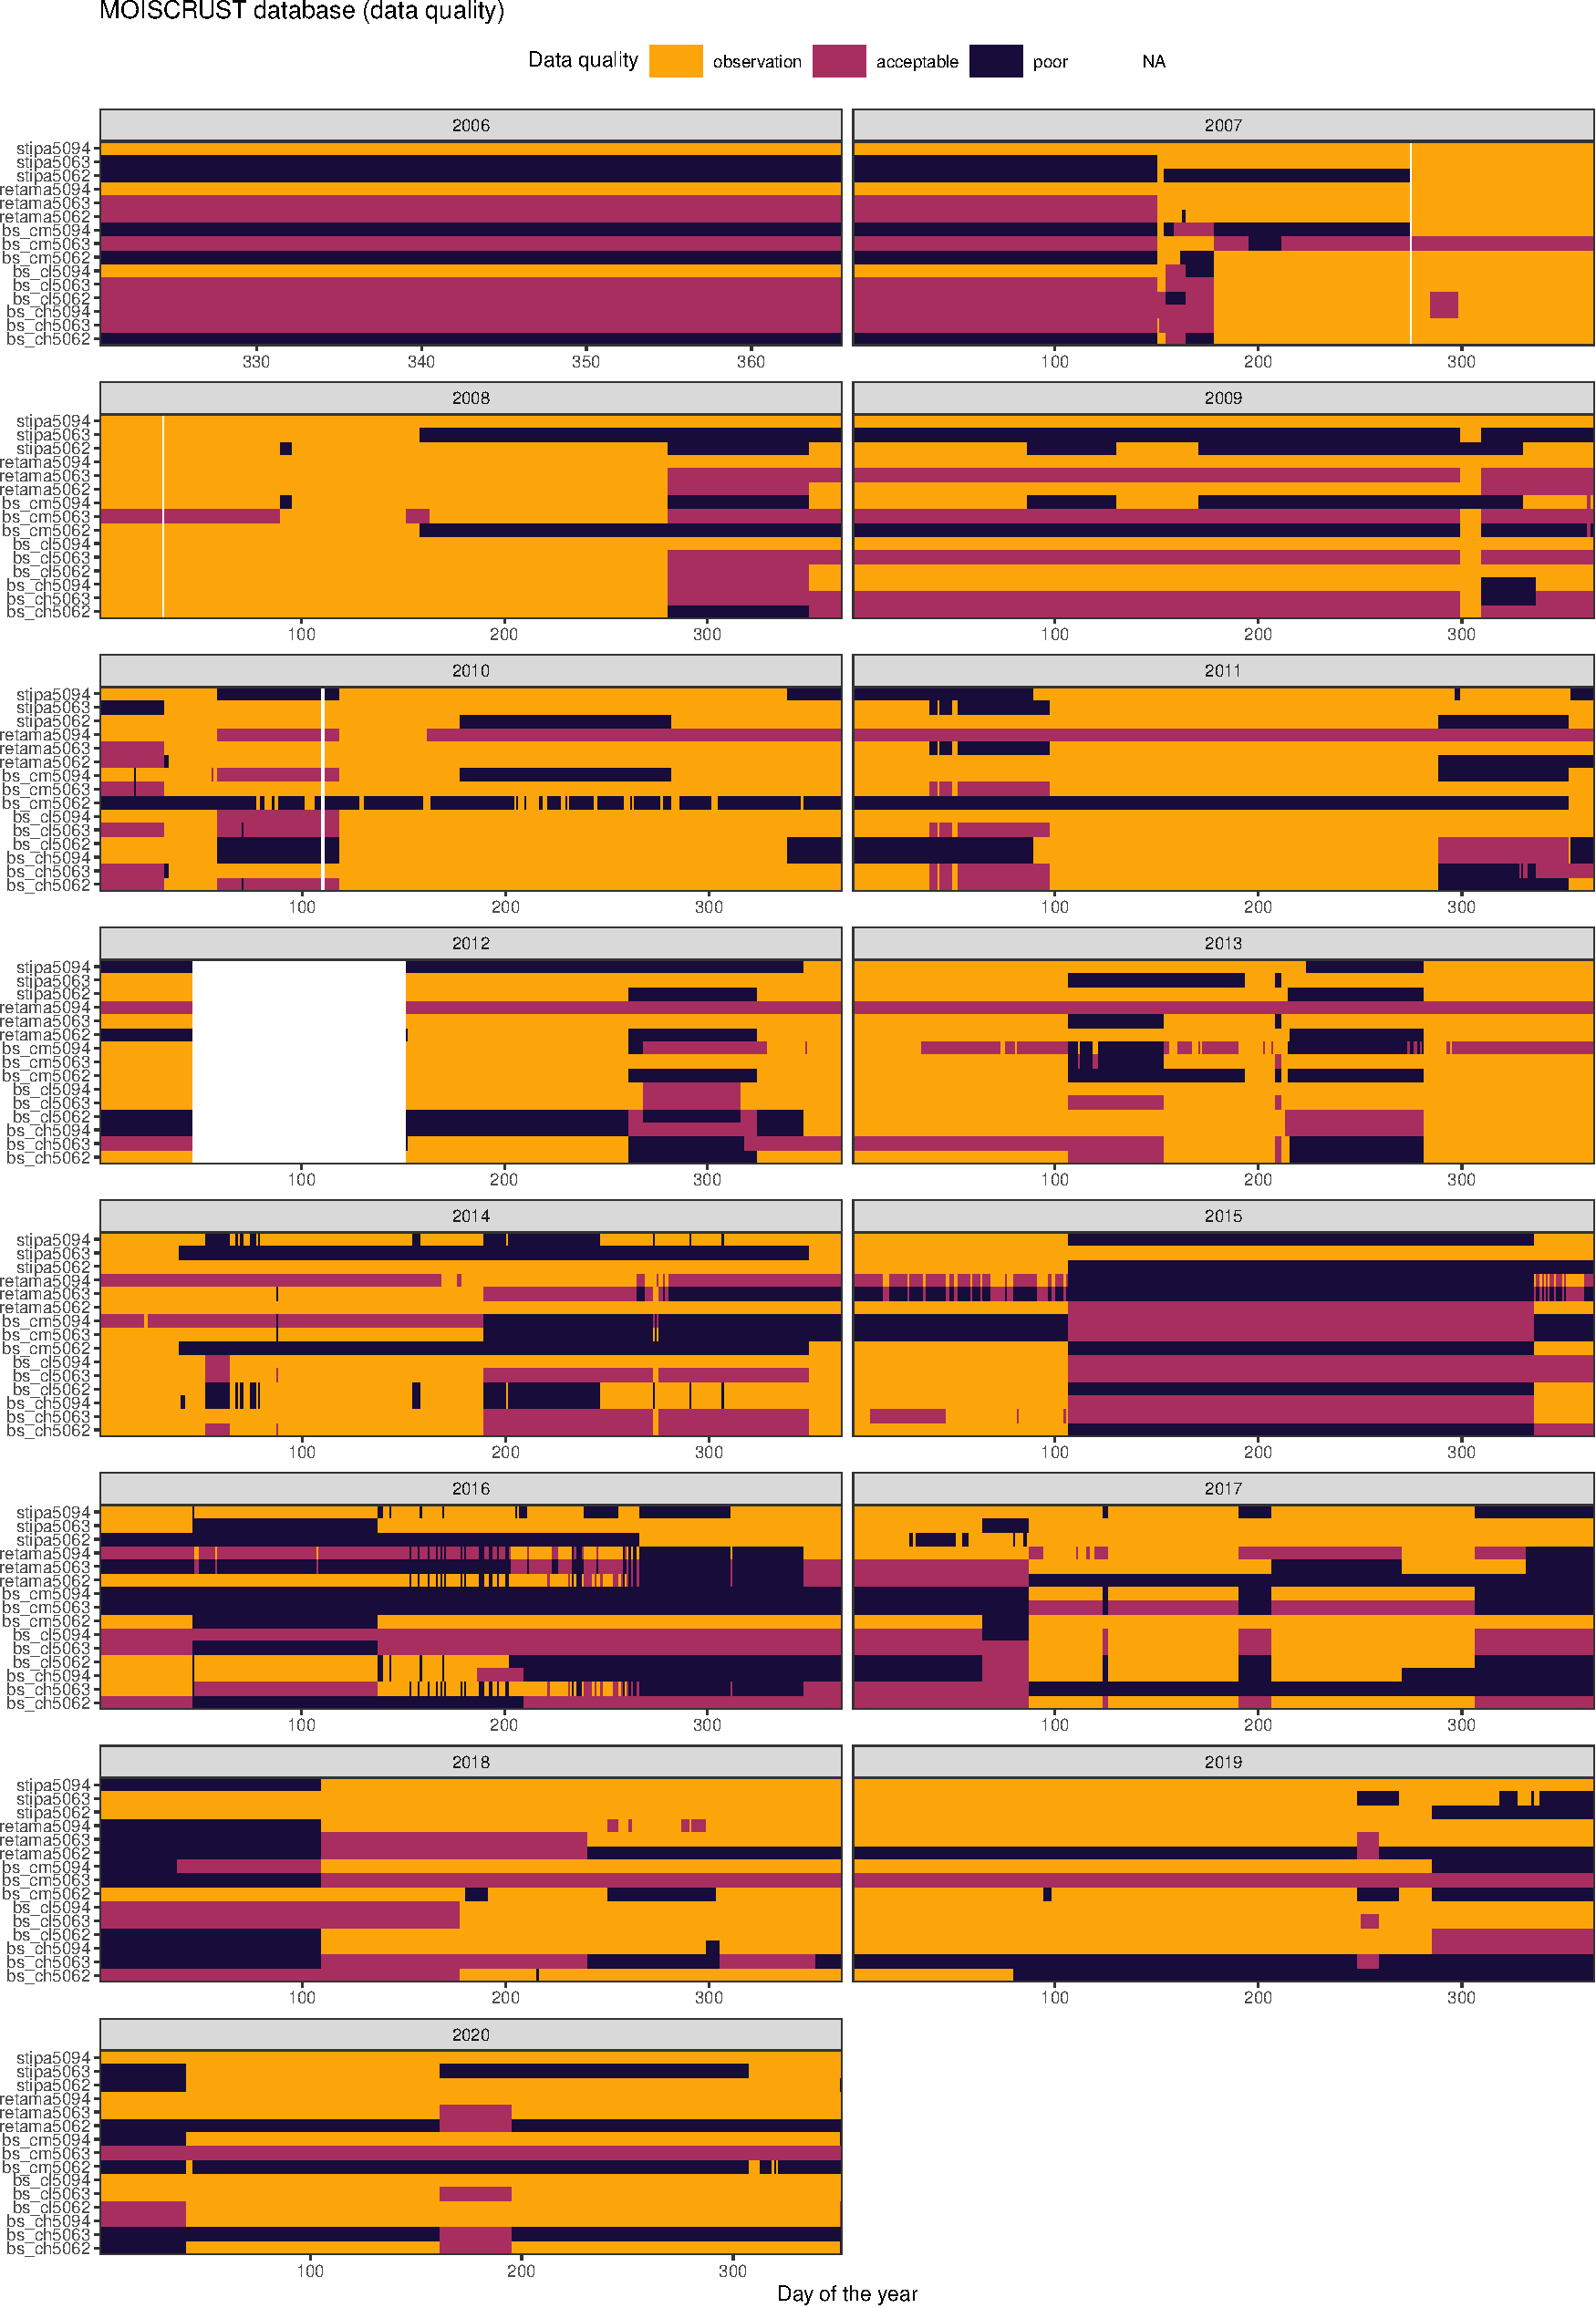
\includegraphics{moiscrust_files/figure-latex/unnamed-chunk-23-1.pdf}

\begin{Shaded}
\begin{Highlighting}[]
\KeywordTok{ggsave}\NormalTok{(}
  \DataTypeTok{width =} \DecValTok{12}\NormalTok{, }
  \DataTypeTok{height =} \DecValTok{17}\NormalTok{, }
  \DataTypeTok{filename =} \StringTok{"MOISCRUST_interpolated_quality.pdf"}
\NormalTok{  )}
\end{Highlighting}
\end{Shaded}

The r squared between the predicted sensor values and the predictor are
shown with transparency. Interpolated records with higher transparency
may have lower quality.

\begin{Shaded}
\begin{Highlighting}[]
\KeywordTok{ggplot}\NormalTok{(moiscrust_long) }\OperatorTok{+}\StringTok{ }
\StringTok{  }\KeywordTok{facet_wrap}\NormalTok{(}
    \StringTok{"year"}\NormalTok{, }
    \DataTypeTok{scales =} \StringTok{"free_x"}\NormalTok{, }
    \DataTypeTok{ncol =} \DecValTok{2}
\NormalTok{    ) }\OperatorTok{+}
\StringTok{  }\KeywordTok{aes}\NormalTok{(}
    \DataTypeTok{x =}\NormalTok{ year_day, }
    \DataTypeTok{y =}\NormalTok{ sensor, }
    \DataTypeTok{fill =}\NormalTok{ soil_moisture}
\NormalTok{    ) }\OperatorTok{+}\StringTok{ }
\StringTok{  }\KeywordTok{geom_tile}\NormalTok{() }\OperatorTok{+}\StringTok{ }
\StringTok{  }\KeywordTok{coord_cartesian}\NormalTok{(}\DataTypeTok{expand =} \OtherTok{FALSE}\NormalTok{) }\OperatorTok{+}
\StringTok{  }\KeywordTok{theme_bw}\NormalTok{() }\OperatorTok{+}\StringTok{ }
\StringTok{  }\KeywordTok{scale_fill_viridis_c}\NormalTok{(}
    \DataTypeTok{direction =} \DecValTok{-1}\NormalTok{, }
    \DataTypeTok{na.value =} \StringTok{"white"}\NormalTok{, }
    \DataTypeTok{option =} \StringTok{"B"}
\NormalTok{    ) }\OperatorTok{+}
\StringTok{  }\KeywordTok{theme}\NormalTok{(}\DataTypeTok{legend.position =} \StringTok{"top"}\NormalTok{) }\OperatorTok{+}\StringTok{ }
\StringTok{  }\KeywordTok{ylab}\NormalTok{(}\StringTok{""}\NormalTok{) }\OperatorTok{+}\StringTok{ }
\StringTok{  }\KeywordTok{xlab}\NormalTok{(}\StringTok{"Day of the year"}\NormalTok{) }\OperatorTok{+}
\StringTok{  }\KeywordTok{ggtitle}\NormalTok{(}\StringTok{"MOISCRUST database (observed and interpolated records)"}\NormalTok{) }\OperatorTok{+}
\StringTok{  }\KeywordTok{labs}\NormalTok{(}\DataTypeTok{fill =} \KeywordTok{expression}\NormalTok{(}\StringTok{"Volumetric water content (cm³ water / cm³ soil)"}\NormalTok{)) }\OperatorTok{+}\StringTok{ }
\StringTok{  }\KeywordTok{theme}\NormalTok{(}\DataTypeTok{legend.key.width =} \KeywordTok{unit}\NormalTok{(}\FloatTok{0.8}\NormalTok{, }\StringTok{"cm"}\NormalTok{))}
\end{Highlighting}
\end{Shaded}

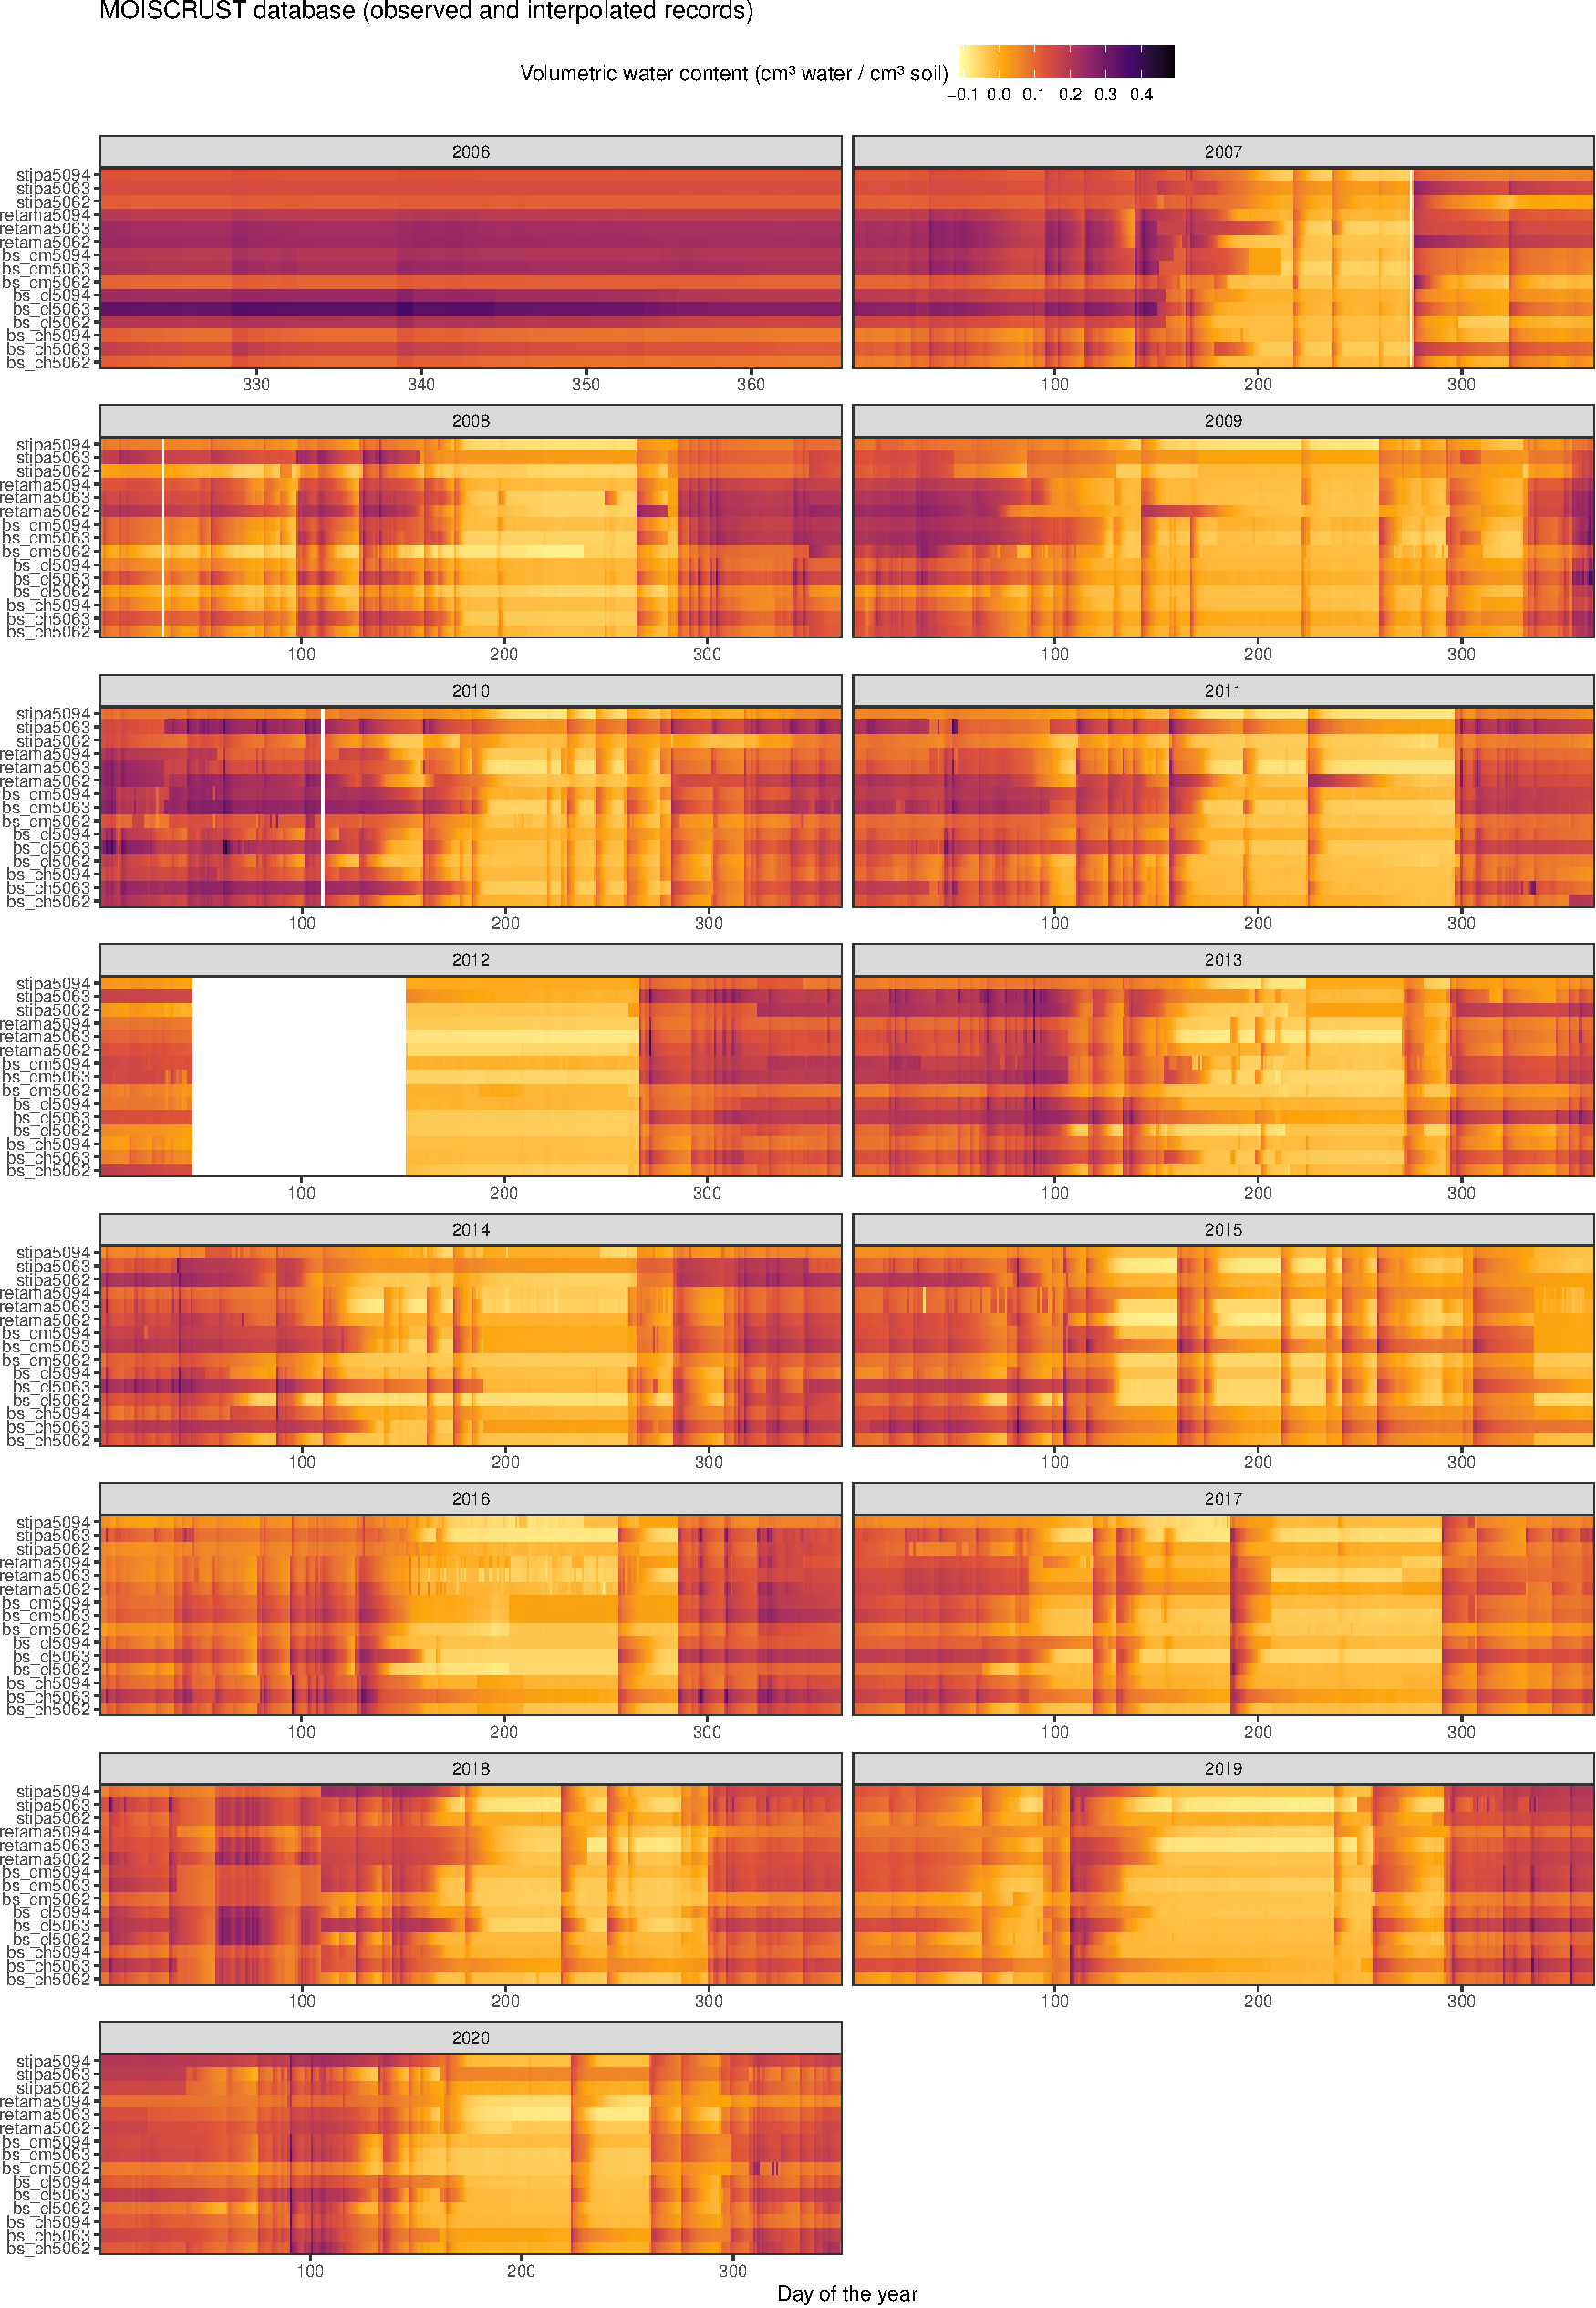
\includegraphics{moiscrust_files/figure-latex/unnamed-chunk-24-1.pdf}

\begin{Shaded}
\begin{Highlighting}[]
\KeywordTok{ggsave}\NormalTok{(}\DataTypeTok{width =} \DecValTok{12}\NormalTok{, }\DataTypeTok{height =} \DecValTok{17}\NormalTok{, }\DataTypeTok{filename =} \StringTok{"MOISCRUST_interpolated.pdf"}\NormalTok{)}
\end{Highlighting}
\end{Shaded}

\hypertarget{data-base-formatting}{%
\section{Data base formatting}\label{data-base-formatting}}

The dataset \texttt{moiscrust\_long} is the database in long format
already.

\begin{tabular}[t]{l|r|l|l|r|r|r|r|r|r|l|r|l|r|r|r|l|l|r|r|r|l|l}
\hline
date\_time & date\_time\_id & date & time & year & year\_day & month & month\_day & week & week\_day & sensor & soil\_moisture & interpolated & model\_estimate & model\_ci\_lower & model\_ci\_upper & model\_predictor & same\_sensor\_group & sensors\_r\_squared & valid\_cases\_shared\_percent & selection\_score & sensor\_group & interpolation\_quality\\
\hline
2006-11-17 18:00:00 & 1 & 2006-11-17 & 18:00 & 2006 & 321 & 11 & 17 & 46 & 6 & retama5094 & 0.1970000 & FALSE & NA & NA & NA & NA & NA & NA & NA & NA & NA & observation\\
\hline
2006-11-17 18:00:00 & 1 & 2006-11-17 & 18:00 & 2006 & 321 & 11 & 17 & 46 & 6 & retama5062 & 0.2442059 & TRUE & 0.2442059 & 0.2422496 & 0.2461622 & retama5094 & TRUE & 0.8825786 & 20.50395 & 208.7618 & retama & acceptable\\
\hline
2006-11-17 18:00:00 & 1 & 2006-11-17 & 18:00 & 2006 & 321 & 11 & 17 & 46 & 6 & retama5063 & 0.2375965 & TRUE & 0.2375965 & 0.2361139 & 0.2390791 & retama5094 & TRUE & 0.9065618 & 28.73605 & 219.3922 & retama & acceptable\\
\hline
2006-11-17 18:00:00 & 1 & 2006-11-17 & 18:00 & 2006 & 321 & 11 & 17 & 46 & 6 & stipa5094 & 0.1320000 & FALSE & NA & NA & NA & NA & NA & NA & NA & NA & NA & observation\\
\hline
2006-11-17 18:00:00 & 1 & 2006-11-17 & 18:00 & 2006 & 321 & 11 & 17 & 46 & 6 & stipa5062 & 0.1167035 & TRUE & 0.1167035 & 0.1153987 & 0.1180083 & stipa5094 & TRUE & 0.5676305 & 53.85591 & 210.6190 & stipa & poor\\
\hline
2006-11-17 18:00:00 & 1 & 2006-11-17 & 18:00 & 2006 & 321 & 11 & 17 & 46 & 6 & stipa5063 & 0.1435911 & TRUE & 0.1435911 & 0.1419916 & 0.1451907 & stipa5094 & TRUE & 0.5162195 & 48.28543 & 199.9074 & stipa & poor\\
\hline
\end{tabular}

Its columns are:

\begin{itemize}
\tightlist
\item
  \texttt{date\_time}: date and time in POSIX format.
\item
  \texttt{date\_time\_id}: integer, unique ID for each value of
  \texttt{date\_time}.
\item
  \texttt{date}: date in format year-month-day.
\item
  \texttt{time}: time in format hour-minute.
\item
  \texttt{year}: integer, year.
\item
  \texttt{year\_day}: integer, day of the year.
\item
  \texttt{month}: integer, month number.
\item
  \texttt{week}: integer, week of the year.
\item
  \texttt{week\_day}: integer, day of the week.
\item
  \texttt{sensor}: character, sensor name.
\item
  \texttt{soil\_moisture}: numeric, soil moisture value in
  \(m^{3} water /m^{3} soil\).
\item
  \texttt{interpolated}: boolean, \texttt{TRUE} for interpolated records
  and \texttt{FALSE} for observations.
\item
  \texttt{model\_estimate}: numeric, prediction of the linear model.
\item
  \texttt{model\_ci\_lower}: numeric, lower bound of the confidence
  interval of the estimate.
\item
  \texttt{model\_ci\_upper}: numeric, upper bound of the confidence
  interval of the estimate.
\item
  \texttt{model\_predictor}: character, name of the sensor used as
  predictor in the linear model.
\item
  \texttt{same\_sensor\_group}: boolean, \texttt{TRUE} if the sensor and
  its predictor are in the same group (``stipa'', ``retama'',
  ``biocrust\_low'', ``biocrust\_medium'', ``biocrust\_high'').
\item
  \texttt{sensors\_r\_squared}: numeric, R squared between
  \texttt{sensor} and \texttt{model\_predictor}.
\item
  \texttt{valid\_cases\_shared\_percent}: numeric, percentage of shared
  valid cases between \texttt{sensor} and \texttt{model\_predictor},
  taking the total number of values in \texttt{date\_time\_id} as
  reference.
\item
  \texttt{selection\_score}: numeric, value used to select the
  \texttt{model\_predictor}, based on the sum of
  \texttt{same\_sensor\_group} (100 if \texttt{TRUE} and 0 if
  \texttt{FALSE}), \texttt{sensors\_r\_squared} multiplied by 100, and
  \texttt{valid\_cases\_shared\_percent}.
\item
  \texttt{interpolation\_quality}: character, with the values
  ``observation'' for observations, ``acceptable'' for interpolated
  values where \texttt{sensors\_r\_squared} is higher than 0.85 and
  \texttt{valid\_cases\_shared\_percent} is higher than 20, and ``poor''
  for interpolated values below at least one of these thresholds.
\end{itemize}

\hypertarget{saving-the-data-base-in-different-formats}{%
\section{Saving the data base in different
formats}\label{saving-the-data-base-in-different-formats}}

To expand its usability as much as possible, we provide the data in four
different formats: .RData, .csv, .xlsx, and SQLite.

\begin{Shaded}
\begin{Highlighting}[]
\CommentTok{#create directory for the database}
\KeywordTok{dir.create}\NormalTok{(}\StringTok{"database"}\NormalTok{)}

\CommentTok{#rename dataset}
\NormalTok{moiscrust <-}\StringTok{ }\NormalTok{moiscrust_long}

\CommentTok{#save as RData}
\KeywordTok{save}\NormalTok{(}
\NormalTok{  moiscrust, }
  \DataTypeTok{file =} \StringTok{"database/moiscrust.RData"}
\NormalTok{  )}

\CommentTok{#save as csv}
\KeywordTok{write_excel_csv}\NormalTok{(}
  \DataTypeTok{x =}\NormalTok{ moiscrust,}
  \DataTypeTok{path =} \StringTok{"database/moiscrust.csv"}
\NormalTok{)}

\CommentTok{#save as excel file}
\KeywordTok{write_xlsx}\NormalTok{(}
  \DataTypeTok{x =}\NormalTok{ moiscrust,}
  \DataTypeTok{path =} \StringTok{"database/moiscrust.xlsx"}
\NormalTok{)}

\CommentTok{#save as SQLite}
\NormalTok{drv <-}\StringTok{ }\KeywordTok{dbDriver}\NormalTok{(}\StringTok{"SQLite"}\NormalTok{)}
\NormalTok{tfile <-}\StringTok{ "database/moiscrust.db"}
\NormalTok{con <-}\StringTok{ }\KeywordTok{dbConnect}\NormalTok{(drv, }\DataTypeTok{dbname =} \StringTok{"database/moiscrust.db"}\NormalTok{)}
\KeywordTok{dbWriteTable}\NormalTok{(con, }\StringTok{"moiscrust"}\NormalTok{, moiscrust, }\DataTypeTok{overwrite =} \OtherTok{TRUE}\NormalTok{)}
\KeywordTok{dbDisconnect}\NormalTok{(con)}

\CommentTok{#compressing the file}
\KeywordTok{zip}\NormalTok{(}
  \DataTypeTok{zipfile =} \StringTok{"database.zip"}\NormalTok{,}
  \DataTypeTok{files =} \StringTok{"database"}
\NormalTok{  )}
\end{Highlighting}
\end{Shaded}

\end{document}
